\documentclass[18pt,xcolor=table]{beamer}
\usepackage{etex}
\reserveinserts{28}
% -----PACKAGES
%\usepackage[shortend,titlenumbered]{algorithm2e}
%\usepackage{algorithmic}
%\usepackage[plain]{algorithm}
\usepackage{multicol}
\usepackage{color}
\usepackage{multirow}
\usepackage{fancybox}
%\usepackage{index}
\usepackage{varioref}
\usepackage{psfrag}
\usepackage{epsfig}
\usepackage{boxedminipage}
\usepackage{graphicx}
\usepackage{rotating}
\usepackage{amsmath}
\usepackage{amssymb}
%\usepackage{amsfont}
\usepackage{latexsym}
\usepackage{alltt}
%\usepackage[small,bf]{caption}
\usepackage{url}
%\usepackage{citesort}
%\usepackage{crop}
\usepackage{array}
\usepackage{subfigure}
\usepackage{dcolumn}

% -----SETLENGTH
%\setlength{\captionmargin}{20pt} 

% -----NEWCOMMANDS
\newcommand{\nc}{\newcommand}
\nc{\mathsm}[1]{\text{\small{$#1$}}}
\nc{\ubar}[1]{\underset{-}{#1}}
\nc{\optype}{\textrm}
\nc{\EQ}[1]{(\ref{eq:#1})}
\nc{\TAB}[1]{\ref{tab:#1}}
\nc{\FIG}[1]{\ref{fig:#1}}
\nc{\SEC}[1]{\ref{sec:#1}}
\nc{\ALG}[1]{\ref{alg:#1}}
\nc{\CHAP}[1]{\ref{chap:#1}}
\nc{\mtrx}[1]{\boldsymbol{\mathbf{#1}}}
\nc{\vctr}[1]{\boldsymbol{\mathbf{#1}}}
\nc{\grad}{\mbox{\boldmath$\nabla$}}
\nc{\gradient}{\textsl{grad}\,}
\nc{\hessian}{\textsl{grad\,}^2}
\nc{\ii}{\iota}
\nc{\dd}{d}
\nc{\ee}{\mathrm{e}}
\nc{\pdiv}[2]{\partial{#1}/\partial{#2}}
\nc{\dpdiv}[2]{\displaystyle{\frac{\partial{#1}}{\partial{#2}}}}
\nc{\ddiv}[2]{\displaystyle{\frac{\dd{#1}}{\dd{#2}}}}
\nc{\inpr}{\hspace{-1pt}\cdot\hspace{-1pt}}
\nc{\IR}{\mathbb{R}}
\nc{\IN}{\mathbb{N}}
\nc{\IZ}{\mathbb{Z}}
\nc{\IC}{\mathbb{C}}
\nc{\half}{\frac{1}{2}}
\nc{\shalf}{\scriptstyle{\half}} 
\nc{\ds}[1]{\displaystyle{#1}}
\nc{\ts}[1]{\textstyle{#1}}
\nc{\sign}{\optype{sign}}
\nc{\spr}{\optype{spr}}
\nc{\dist}{\optype{dist}}
\nc{\rank}{\optype{rank}}
\nc{\codim}{\optype{codim}}
\nc{\supp}{\optype{supp}}
\nc{\diag}{\optype{diag}}
\nc{\meas}{\optype{meas}}
\nc{\cond}{\optype{cond}}
\nc{\kernel}{\optype{kernel}}
\nc{\spa}{\optype{span}}
\nc{\order}{\mathcal{O}}
\nc{\Fr}{\mathrm{Fr}}
\nc{\Rey}{\mathrm{Re}}
\nc{\Ord}{O}
\nc{\ord}{o}
\nc{\st}{\:{:}\:}
\nc{\closure}[1]{\overline{#1}}
\nc{\emin}[1]{\emph{#1}\index{#1}\/}
\nc{\rmin}[1]{#1\index{{}@{#1}}}
\nc{\Laplace}{\Delta}
\nc{\ie}{i.e.}
\nc{\eg}{e.g.}
%\nc{\union}{\cup}
\nc{\Union}{\bigcup}
\nc{\lf}[1]{\mathsf{#1}}
\nc{\dbar}[1]{\bar{\bar{#1}}}
\nc{\ul}[1]{\underline{#1}}
\nc{\hpt}{\hspace{0.5pt}}
\nc{\E}[1]{\times{}10^{#1}}
\nc{\inp}[2]{\langle{#1},{#2}\rangle}
\nc{\tmpcommand}{}

% -----RENEWCOMMANDS
\renewcommand{\baselinestretch}{1}
\renewcommand{\exp}{\optype{exp}\,}
\renewcommand{\cosh}{\optype{cosh}\,}
\renewcommand{\tanh}{\optype{tanh}\,}
\renewcommand{\sinh}{\optype{sinh}\,}
\renewcommand{\div}[1]{\optype{div}\,{#1}}
\renewcommand{\half}{\mbox{$\frac{1}{2}$}}
%\renewcommand{\descriptionlabel}[1]{\hspace{\labelsep}\emph{#1}}

% -----ETC
\raggedbottom


\DeclareMathOperator{\curl}{\bf curl}
\DeclareMathOperator{\rot}{\rm curl}
\DeclareMathOperator{\divv}{\rm div}
\newcommand{\tro}{\gamma_0}
\newcommand{\trt}{\gamma_{\sft}}
\newcommand{\trn}{\gamma_{\sfn}}

\newcommand{\PT}{{\partial T}}
\newcommand{\bbN}{{\mathbb{N}}}
\newcommand{\bbP}{{\mathbb{P}}}

\newcommand{\scC}{{\mathscr{C}}}
\newcommand{\caD}{{\mathcal{D}}}
\newcommand{\caL}{{\mathcal{L}}}

\newcommand{\sfe}{{\mathsf{e}}}
\newcommand{\sff}{{\mathsf{f}}}
\newcommand{\sft}{{\boldsymbol{\mathsf{t}}}}
\newcommand{\sfn}{{\boldsymbol{\mathsf{n}}}}

%   Common caligraphic abbrevs
\newcommand{\BB}{\mathcal{B}}
\newcommand{\CC}{\mathcal{C}}
\newcommand{\DD}{\mathcal{D}}
\newcommand{\EE}{\mathcal{E}}
\newcommand{\FF}{\mathcal{F}}
\newcommand{\GG}{\mathcal{G}}
\newcommand{\II}{\mathcal{I}}
\newcommand{\JJ}{\mathcal{J}}
\newcommand{\KK}{\mathcal{K}}
\newcommand{\LL}{\mathcal{L}}
\newcommand{\OO}{\mathcal{O}}
\newcommand{\QQ}{\mathcal{Q}}
\newcommand{\RR}{\mathcal{R}}
\newcommand{\TT}{\mathcal{T}}


 %% JAY'S PREAMBLE
 %%========================

%   Math symbol definitions
\def\d{\partial}
%\newsymbol\lee 132E
\newcommand{\union}{\mathop{\bigcup}}
\newcommand{\intersect}{\mathop{\bigcap}}
\newcommand{\binomial}[2]{\ensuremath{
		\begin{pmatrix}{#1}\\{#2}\end{pmatrix}}}
\newcommand{\smallbinomial}[2]{\ensuremath{
		(\begin{smallmatrix}{#1}\\{#2}\end{smallmatrix})}}
\newcommand{\tang}[1]{\ensuremath{{#1}_{\intercal}}} % can use \top
						     % also
\newcommand{\hypergeom}[2]{\ensuremath{\sideset{_{#1}}{_{#2}}{\mathop{F}}}}
%   Difficult names
\newcommand{\Babuska}{Babu{\v{s}}ka}       % Remember: Usage is \Babuska\
\newcommand{\Cea}{C{\'e}a}                 % with trailing `\' to give space
\newcommand{\Poincare}{Poincar{\'{e}}}     % when needed, but when ending
\newcommand{\Nedelec}{N{\'{e}}d{\'{e}}lec} % sentence use \Babuska.
\newcommand{\Frechet}{Fr{\'{e}}chet}
\newcommand{\Muller}{M{\"u}ller}
\newcommand{\LHospital}{L'H{\^{o}}spital}
%   Bold and beautiful
\newcommand{\ba}{{\boldsymbol{a}}}
\newcommand{\bA}{\boldsymbol{A}}
\newcommand{\balpha}{{\boldsymbol{\alpha}}}
\newcommand{\bB}{{\boldsymbol{B}}}
\newcommand{\bb}{{\boldsymbol{b}}}
\newcommand{\bbeta}{{\boldsymbol{\beta}}}
\newcommand{\etab}{{\boldsymbol{\eta}}}
\newcommand{\bC}{{\boldsymbol{C}}}
\newcommand{\bc}{{\boldsymbol{c}}}
\newcommand{\bD}{{\boldsymbol{D}}}
\newcommand{\bd}{{\boldsymbol{d}}}
\newcommand{\db}{{\boldsymbol{\d}}}
\newcommand{\bdelta}{{\boldsymbol{\delta}}}
\newcommand{\bDelta}{{\boldsymbol{\Delta}}}
\newcommand{\beps}{{\boldsymbol{\varepsilon}}}
\newcommand{\be}{{\boldsymbol{e}}}
\newcommand{\bg}{{\boldsymbol{g}}}
\newcommand{\bm}{{\boldsymbol{m}}}
\newcommand{\bn}{{\boldsymbol{n}}}
\newcommand{\bN}{{\boldsymbol{N}}}
\newcommand{\bp}{{\boldsymbol{p}}}
\newcommand{\bpsi}{{\boldsymbol{\psi}}}
\newcommand{\bq}{{\boldsymbol{q}}}
\newcommand{\bxi}{{\boldsymbol{\xi}}}
\newcommand{\bE}{{\boldsymbol{E}}}
\newcommand{\bF}{{\boldsymbol{F}}}
\newcommand{\bh}{{\boldsymbol{h}}}
\newcommand{\bH}{{\boldsymbol{H}}}
\newcommand{\bI}{{\boldsymbol{I}}}
\newcommand{\bj}{{\boldsymbol{j}}}
\newcommand{\bJ}{{\boldsymbol{J}}}
\newcommand{\bK}{{\boldsymbol{K}}}
\newcommand{\bk}{{\boldsymbol{k}}}
\newcommand{\bll}{{\boldsymbol{\ell}}}
\newcommand{\bL}{{\boldsymbol{L}}}
\newcommand{\blambda}{{\boldsymbol{\lambda}}}
\newcommand{\bmu}{{\boldsymbol{\mu}}}
\newcommand{\bM}{{\boldsymbol{M}}}
\newcommand{\bomega}{{\boldsymbol{\omega}}}
\newcommand{\bP}{{\boldsymbol{P}}}
\newcommand{\bphi}{{\boldsymbol{\phi}}}
\newcommand{\bQ}{{\boldsymbol{Q}}}
\newcommand{\bG}{{\boldsymbol{G}}}
\newcommand{\bu}{{\boldsymbol{u}}}
\newcommand{\bU}{{\boldsymbol{U}}}
\newcommand{\bV}{{\boldsymbol{V}}}
\newcommand{\bX}{{\boldsymbol{X}}}
\newcommand{\bv}{{\boldsymbol{v}}}
\newcommand{\bw}{{\boldsymbol{w}}}
\newcommand{\bW}{{\boldsymbol{W}}}
\newcommand{\bR}{{\boldsymbol{R}}}
\newcommand{\br}{{\boldsymbol{r}}}
\newcommand{\bS}{{\boldsymbol{S}}}
\newcommand{\bT}{{\boldsymbol{T}}}
\newcommand{\btau}{{\boldsymbol{\tau}}}
\newcommand{\bt}{{\boldsymbol{t}}}
\newcommand{\bx}{{\boldsymbol{x}}}
\newcommand{\by}{{\boldsymbol{y}}}
\newcommand{\bz}{{\boldsymbol{z}}}
\newcommand{\bzero}{{\boldsymbol{0}}}
\newcommand{\bZ}{{\boldsymbol{Z}}}
%   Common scalar fields
\newcommand{\RRR}{\mathbb{R}}
\newcommand{\CCC}{\mathbb{C}}
\newcommand{\ZZZ}{\mathbb{Z}}
\newcommand{\NNN}{\mathbb{N}}
%   Differential operators
\newcommand{\dive}{\mathop\mathrm{div}}
%\newcommand{\grad}{\ensuremath{\mathop{{\bf{grad}}}}}
%\newcommand{\curl}{{\ensuremath\mathop{\mathbf{curl}\,}}}
\newcommand{\Curl}{ {\bf Curl}}
\newcommand{\dx}{\ensuremath{\mathrm{d}x}}
\newcommand{\dy}{\ensuremath{\mathrm{d}y}}
\newcommand{\dr}{\ensuremath{\mathrm{d}r}}
\newcommand{\dR}{\ensuremath{\mathrm{d}R}}
\newcommand{\drho}{\ensuremath{\mathrm{d}\rho}}
\newcommand{\dz}{\ensuremath{\mathrm{d}z}}
\newcommand{\dzeta}{\ensuremath{\mathrm{d}\zeta}}
%   Wordy math symbols
\newcommand{\card}{\ensuremath{\mathop\mathrm{card}}}
%\newcommand{\diag}{\ensuremath{\mathop\mathrm{diag}}}
\newcommand{\diam}{\ensuremath{\mathop\mathrm{diam}}}
%\newcommand{\dist}{\mathop\mathrm{dist}}
\newcommand{\Ker}{\mathop\mathrm{Ker}}
\newcommand{\Range}{\mathop\mathrm{Range}}
%\newcommand{\rank}{\mathop\mathrm{rank}}
%\newcommand{\meas}{\mathop\mathrm{meas}}
\newcommand{\Forall}{\quad\text{for all }}
%\newcommand{\supp}{\mathop\mathrm{supp}}
\newcommand{\Span}{\mathop\mathrm{Span}}
\newcommand{\Hdiv}[1]{\bH(\dive,#1)}
%\newcommand{\Hcurl}[1]{\bH(\curl,#1)}
%   Common caligraphic abbrevs
%\newcommand{\BB}{\mathcal{B}}
%\newcommand{\CC}{\mathcal{C}}
%\newcommand{\DD}{\mathcal{D}}
%\newcommand{\EE}{\mathcal{E}}
%\newcommand{\FF}{\mathcal{F}}
%\newcommand{\GG}{\mathcal{G}}
%\newcommand{\II}{\mathcal{I}}
%\newcommand{\JJ}{\mathcal{J}}
%\newcommand{\KK}{\mathcal{K}}
%\newcommand{\LL}{\mathcal{L}}
%\newcommand{\OO}{\mathcal{O}}
%\newcommand{\QQ}{\mathcal{Q}}
%\newcommand{\RR}{\mathcal{R}}
%\newcommand{\TT}{\mathcal{T}}
%   Variations on standard symbols
\newcommand{\veps}{\varepsilon}
\newcommand{\vlam}{\varLambda}
\newcommand{\vpi}{\varPi}
\newcommand{\vPi}{\boldsymbol{\varPi}}
\newcommand{\vsig}{\varSigma}
\newcommand{\vbt}{\boldsymbol{\varTheta}}
\newcommand{\vPsi}{\boldsymbol{\varPsi}}
%\newcommand{\ii}{\hat{\imath}}
%   Innerproducts, norms, etc
\newcommand{\ntrip}[1]{|\!|\!| {#1} |\!|\!|}
\newcommand{\ip}[1]{\langle {#1} \rangle}
%   Utilities
\newcommand{\blnk}{\underline{\hspace{3cm}}\;}
\newcommand{\marg}[1]{\marginpar{\tiny{\framebox{\parbox{1.7cm}{#1}}}}}
\newcommand{\degreeC}[1]{\ensuremath{{#1\,}^\circ\!\text{C}}}
                        % try also  \textcelsius of textcomp package
%   Trademarked names \texttrademark, \textregistered
\newcommand{\matlab}{MATLAB\textregistered\renewcommand{\matlab}{MATLAB}}
\newcommand{\femlab}{FEMLAB\textregistered\renewcommand{\femlab}{FEMLAB}}

%   Style preferences
\renewcommand{\thefootnote}{\fnsymbol{footnote}} % Use symbols instead of
						 % numbers for footnotes
						 

\newcommand{\Eg}{\EE^\mathrm{grad}}
\newcommand{\Ec}{\boldsymbol{\EE}^\mathrm{curl}}
\newcommand{\Ed}{\boldsymbol{\EE}^\mathrm{div}}


\newcommand{\bfdu}{\mbox{\boldmath $\delta u$}}
\newcommand{\bfdv}{\mbox{\boldmath $\delta v$}}
\newcommand{\du}{{\delta u}}
\newcommand{\dv}{{\delta v}}
\newcommand{\bfnabt}{\widetilde{\bfnab}}
\newcommand{\bfepst}{\widetilde{\bfeps}}

\graphicspath{{../Proposal/figs/}{../PD13/figs/}{../Figures/}}

\usepackage{bbm}
\usepackage{textpos}
\usepackage{pgf,tikz}
\usepackage{pgfplots}
\usepackage[space]{grffile}
\usepackage{graphicx}
\usepackage{forloop}
% \usepackage[aps,prb,citeautoscript]{revtex4-1}
% \usepackage[super]{natbib}
\usepackage[backend=bibtex,sorting=none]{biblatex}
\usepackage{animate}
\usepackage{listings}
\usepackage{bbding}
\usepackage{comment}
\bibliography{../Papers}

\newcounter{nn}

% \AtBeginSection[]
% {
%   \begin{frame}
%     \frametitle{Table of Contents}
%     \framesubtitle{\hspace{1ex}}
%     \tableofcontents[currentsection,currentsubsection]
%   \end{frame}
% }
% \AtBeginSubsection[] {
%   \begin{frame}
%     \frametitle{Table of Contents}
%     \framesubtitle{\hspace{1ex}}
%     \tableofcontents[currentsection,currentsubsection]
%   \end{frame}
% }

\definecolor{utorange}{RGB}{203,96,21}
\definecolor{utblack}{RGB}{99,102,106}
\definecolor{utbrown}{RGB}{110,98,89}
\definecolor{utsecbrown}{RGB}{217,200,158}
\definecolor{utsecgreen}{RGB}{208,222,187}
\definecolor{utsecblue}{RGB}{127,169,174}

\mode<presentation>
{
  % \usetheme{Pittsburgh}
  \usetheme{Boadilla}
  \usefonttheme[onlymath]{serif}

  \setbeamercovered{invisible}
  \setbeamertemplate{navigation symbols}{}

  % Color Theme
    \setbeamercolor{normal text}{bg=white,fg=utblack}
  \setbeamercolor{structure}{fg=utorange}

  \setbeamercolor{alerted text}{fg=red!85!black}

  \setbeamercolor{item projected}{use=item,fg=black,bg=item.fg!35}

  \setbeamercolor*{palette primary}{use=structure,fg=white, bg=utorange}
  \setbeamercolor*{palette secondary}{use=structure,bg=utsecbrown}
  \setbeamercolor*{palette tertiary}{use=structure,bg=utsecgreen}
  \setbeamercolor*{palette quaternary}{use=structure,fg=structure.fg,bg=utsecblue}

  % \setbeamercolor*{frametitle}{use=structure,fg=utorange, bg=utsecbrown}
  \setbeamercolor*{framesubtitle}{fg=utbrown}

  \setbeamercolor*{block title}{parent=structure,fg=black,bg=utsecgreen}
  \setbeamercolor*{block body}{fg=black,bg=utblack!10}
  \setbeamercolor*{block title alerted}{parent=alerted text,bg=black!15}
  \setbeamercolor*{block title example}{parent=example text,bg=black!15}

  \setbeamerfont{framesubtitle}{size=\small}
}

% \usepackage[orientation=landscape,size=custom,width=16,height=9.75,scale=0.5,debug]{beamerposter}
% \usepackage[orientation=landscape,size=custom,width=16,height=9,scale=0.5,debug]{beamerposter}


\makeatletter
\setbeamertemplate{footline}
{
  \leavevmode%
    \hbox{%
      \begin{beamercolorbox}[wd=.333333\paperwidth,ht=2.25ex,dp=1ex,center]{author in head/foot}%
        \usebeamerfont{author in head/foot}\insertshortauthor%~~\beamer@ifempty{\insertshortinstitute}{}{(\insertshortinstitute)}
      \end{beamercolorbox}%
        \begin{beamercolorbox}[wd=.333333\paperwidth,ht=2.25ex,dp=1ex,center]{title in head/foot}%
        \usebeamerfont{title in head/foot}\insertshorttitle
        \end{beamercolorbox}%
        \begin{beamercolorbox}[wd=.333333\paperwidth,ht=2.25ex,dp=1ex,right]{date in head/foot}%
        \usebeamerfont{date in head/foot}\insertshortdate{}\hspace*{2em}
        \insertframenumber{} / \inserttotalframenumber\hspace*{2ex}
      \end{beamercolorbox}}%
        \vskip0pt%
}
\makeatother

\usepackage{kerkis}
\usepackage[T1]{fontenc}
\usepackage[protrusion=true,expansion=true]{microtype}
\usepackage{amsmath}


\renewcommand*{\thefootnote}{\fnsymbol{footnote}}

\let\oldfootnotesize\footnotesize
\renewcommand*{\footnotesize}{\oldfootnotesize\tiny}


\pgfdeclareimage[height=1.2cm]{utbig}{logos/UTWordmark}
\pgfdeclareimage[height=0.6cm]{ut}{logos/UTWordmark}
% \pgfdeclareimage[height=10.0cm]{utbig}{logos/ICES-wordmark-teal.pdf}
% \pgfdeclareimage[height=0.6cm]{ut}{logos/ICES-wordmark-teal.pdf}
% \pgfdeclareimage[height=1.5cm]{iceslogo}{logos/ICES-wordmark-teal.png}
% \pgfdeclareimage[height=1.0cm]{scsmall}{logos/SC12}

\title[Robust Norms for Space-Time Fluid Flow]{Robust DPG Test Norms for Space-Time Convection-Diffusion}
% \subtitle{If you have one}
\author[Truman E. Ellis]{ \underline{Truman~Ellis} \\
{\oldfootnotesize \smallskip Advisors: Leszek Demkowicz, Robert Moser, \\Collaborators: Nate Roberts (Argonne), Jesse Chan (Virginia Tech)}
}

\begin{comment}
The discontinuous Petrov-Galerkin method is a novel finite element framework with exceptional stability and adaptivity properties.
The DPG framework can be used to derive stable discretizations of any well-posed variational formulation 
and has been successfully applied to problems such as heat conduction, time-harmonic Helmholtz, 
Maxwell's equations, linear elasticity and plate problems, Stokes flow, and both incompressible and compressible Navier-Stokes.
In contrast to many other numerical methods, DPG does not suffer from a pre-asymptotic regime (unstable behavior on coarse meshes).
This means that a simulation can be initiated at the coarsest scale possible while automatic adaptivity resolves solution features 
based on a robust, built-in measure of residual error.
DPG is intensely locally compute intensive with significant embarrassingly parallel computations done both pre- and post-global solve.
We present preliminary work on a space-time DPG formulation that enables automatic local time stepping and a kind of parallel-in-time integration.
We also present the Camellia library, which is built on top of Trilinos and 
supports rapid specification of DPG problems while maintaining computational efficiency and scalability.
\end{comment}

% \institute{Institute for Computational Engineering \& Sciences\\ \mbox{}  \\  \pgfuseimage{utbig} }
\institute{
\large{FEM Rodeo 2016}
\vspace{4ex}

\pgfuseimage{utbig}
\\ \vspace{2ex}

\includegraphics[trim=3.0in 7.2in 1.5in 4.0in,width=0.3\linewidth]{logos/ICES-wordmark-teal.pdf}
}
\date[FEM Rodeo 2016]%{\pgfuseimage{iceslogo} }

\begin{document}
\def\thefootnote{\arabic{footnote}}

\tikzstyle{block} = [rectangle, draw, rounded corners, shade, top color=white, text width=5em,
  bottom color=blue!50!black!20, draw=blue!40!black!60, very thick, text centered, minimum height=4em]
  \tikzstyle{line} = [draw, -latex']
  \tikzstyle{cloud} = [draw, ellipse,top color=white, bottom color=red!20, node distance=2cm, minimum height=2em]


  \beamertemplateballitem
  %\beamertemplatetransparentcoveredhigh

  \frame{\titlepage}

  \addtobeamertemplate{frametitle}{}{%
      \begin{textblock*}{100mm}(0.87\textwidth,-0.75cm)
    \pgfuseimage{ut}
    \end{textblock*}
  }



%   /$$$$$$$  /$$$$$$$   /$$$$$$         /$$$$$$                                            /$$                        
%  | $$__  $$| $$__  $$ /$$__  $$       /$$__  $$                                          |__/                        
%  | $$  \ $$| $$  \ $$| $$  \__/      | $$  \ $$ /$$    /$$  /$$$$$$   /$$$$$$  /$$    /$$ /$$  /$$$$$$  /$$  /$$  /$$
%  | $$  | $$| $$$$$$$/| $$ /$$$$      | $$  | $$|  $$  /$$/ /$$__  $$ /$$__  $$|  $$  /$$/| $$ /$$__  $$| $$ | $$ | $$
%  | $$  | $$| $$____/ | $$|_  $$      | $$  | $$ \  $$/$$/ | $$$$$$$$| $$  \__/ \  $$/$$/ | $$| $$$$$$$$| $$ | $$ | $$
%  | $$  | $$| $$      | $$  \ $$      | $$  | $$  \  $$$/  | $$_____/| $$        \  $$$/  | $$| $$_____/| $$ | $$ | $$
%  | $$$$$$$/| $$      |  $$$$$$/      |  $$$$$$/   \  $/   |  $$$$$$$| $$         \  $/   | $$|  $$$$$$$|  $$$$$/$$$$/
%  |_______/ |__/       \______/        \______/     \_/     \_______/|__/          \_/    |__/ \_______/ \_____/\___/ 
%                                                                                                                      
%                                                                                                                      
% 
\section{DPG: A Framework for Computational Mechanics}

% % ------------------------------------------------------------
% \begin{frame}[t]
% \frametitle{Overview of DPG}
% \framesubtitle{A Framework for Automated Scientific Computing}
% Overview of Features
% \begin{itemize}
% \item Provides a framework for developing stable finite element methods
% \item Robust for singularly perturbed problem
% \item Stable in the pre-asymptotic regime
% \item Residual measure drives adaptivity
% \item Hermitian positive-definite stiffness matrix
% \end{itemize}
% \end{frame}



% ------------------------------------------------------------
\begin{frame}[t]
\frametitle{Overview of DPG}
\framesubtitle{A Framework for Computational Mechanics}
Find $u\in U$ such that
\[
b(u,v)=l(v)\quad\forall v\in V
\]
with operator $B:U\rightarrow V'$ defined by $b(u,v)=\LRa{Bu,v}_{V'\times V}$.

This gives the operator equation 
\[
Bu=l\quad\in V'\,.
\]
We wish to minimize the residual $Bu-l\in V'$:
\[
u_h=\argmin_{w_h\in U_h}\frac{1}{2}\norm{Bw_h-l}^2_{V'}\,.
\]
Dual norms are not computationally tractable. 
Inverse Riesz map moves the residual to a more accessible space:
\[
u_h=\argmin_{w_h\in U_h}\frac{1}{2}\norm{R_V^{-1}(Bw_h-l)}^2_{V}\,.
\]
\end{frame}


% ------------------------------------------------------------
\begin{frame}[t]
\frametitle{Overview of DPG}
\framesubtitle{Petrov-Galerkin with Optimal Test Functions}
% \framesubtitle{Optimal Petrov-Galerkin Methods}
Taking the G\^ateaux derivative to be zero in all directions $\delta u \in
U_h$ gives,
\[
\left(R_V^{-1}(Bu_h-l),R_V^{-1}B\delta u\right)_V = 0, \quad \forall \delta u \in U,
\]
which by definition of the Riesz map is equivalent to 
\begin{equation*}
\LRa{Bu_h-l,R_V^{-1}B\delta u_h}=0\quad\forall\delta u_h\in U_h\,,
\end{equation*}
with optimal test functions $v_{\delta u_h}\coloneqq R_V^{-1}B\delta u_h$ for each trial function $\delta u_h$.
\begin{block}{Resulting Petrov-Galerkin System}
This gives a simple bilinear form
\begin{equation*}
b(u_h,v_{\delta u_h})=l(v_{\delta u_h}),
\end{equation*}
with $v_{\delta u_h}\in V$ that solves the auxiliary problem
\begin{equation*}
\LRp{v_{\delta u_h},\delta v}_V=\LRa{R_Vv_{\delta u_h},\delta v}
=\LRa{B\delta u_h,\delta v}=b(\delta u_h,\delta v)\quad\forall\delta v\in V.
\end{equation*}
\end{block}
\end{frame}






%    /$$$$$$                                                  /$$$$$$$$ /$$                        
%   /$$__  $$                                                |__  $$__/|__/                        
%  | $$  \__/  /$$$$$$   /$$$$$$   /$$$$$$$  /$$$$$$            | $$    /$$ /$$$$$$/$$$$   /$$$$$$ 
%  |  $$$$$$  /$$__  $$ |____  $$ /$$_____/ /$$__  $$ /$$$$$$   | $$   | $$| $$_  $$_  $$ /$$__  $$
%   \____  $$| $$  \ $$  /$$$$$$$| $$      | $$$$$$$$|______/   | $$   | $$| $$ \ $$ \ $$| $$$$$$$$
%   /$$  \ $$| $$  | $$ /$$__  $$| $$      | $$_____/           | $$   | $$| $$ | $$ | $$| $$_____/
%  |  $$$$$$/| $$$$$$$/|  $$$$$$$|  $$$$$$$|  $$$$$$$           | $$   | $$| $$ | $$ | $$|  $$$$$$$
%   \______/ | $$____/  \_______/ \_______/ \_______/           |__/   |__/|__/ |__/ |__/ \_______/
%            | $$                                                                                  
%            | $$                                                                                  
%            |__/  


% ------------------------------------------------------------
\begin{frame}[t]
\frametitle{Space-Time DPG}
\framesubtitle{Extending DPG to Transient Problems}
\begin{itemize}
  \item Time stepping techniques are not ideally suited to highly adaptive grids
  \item Space-time FEM proposed as a solution
  \begin{itemize}
    \item[\textcolor{green}{\Checkmark}] Unified treatment of space and time
    \item[\textcolor{green}{\Checkmark}] Local space-time adaptivity (local time stepping)
    \item[\textcolor{green}{\Checkmark}] Parallel-in-time integration (space-time multigrid)
    \item[\XSolidBrush] Spatially stable FEM methods may not be stable in space-time
    \item[\XSolidBrush] Need to support higher dimensional problems
  \end{itemize}
  \item DPG provides necessary stability and adaptivity
\end{itemize}
\begin{figure}[b]
\centering
% 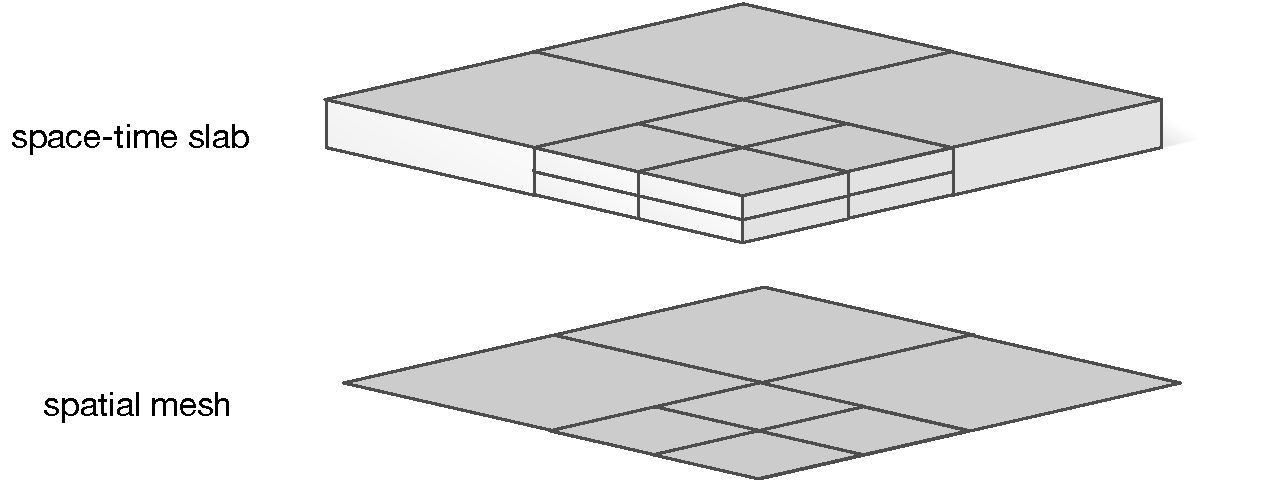
\includegraphics[width=0.8\textwidth]{Schematics/SpaceTimeSchematic}
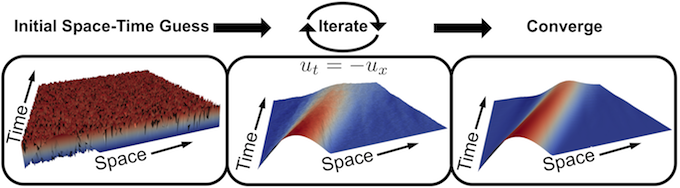
\includegraphics[width=1.0\textwidth]{Schematics/XBraid}
\\\small{Courtesy XBraid by LLNL}
\end{figure}
\end{frame}


\section{Space-Time Model Problem}
% ------------------------------------------------------------
\begin{frame}[t]
\frametitle{Space-Time DPG for Convection-Diffusion}
\framesubtitle{Space-Time Divergence Form}
Equation is parabolic in space-time.
\[
\pd{u}{t}+\bfbeta\cdot\Grad u-\epsilon\Delta u=f
\]
This is just a composition of a constitutive law and conservation of mass.
\begin{align*}
\bfsigma-\epsilon\Grad u&=0\\
\pd{u}{t}+\Div\LRp{\bfbeta u-\bfsigma}&=f
\end{align*}

We can rewrite this in terms of a space-time divergence.
\begin{align*}
\frac{1}{\epsilon}\bfsigma-\Grad u &=0\\
\Gradxt\cdot\vecttwo{\bfbeta u-\bfsigma}{u}&=f
\end{align*}
\end{frame}


% ------------------------------------------------------------
\begin{frame}[t]
\frametitle{Space-Time DPG for Convection-Diffusion}
\framesubtitle{Ultra-Weak Formulation with Discontinuous Test Functions}  %% needed for proper positioning of the logo ...
% \vspace{-2ex}
Multiply by test function and integrate by parts over space-time element K.
\begin{equation*}
\begin{aligned}
\LRp{\frac{1}{\epsilon}\bfsigma,\bftau}_K+\LRp{u,\Div\bftau}_K-\LRa{\hat u,\bftau\cdot\bfn_x}_{\partial K}&=0\\
-\LRp{\vecttwo{\bfbeta u-\bfsigma}{u},\Gradxt v}_K+\LRa{\hat t,v}_{\partial K}&=f
\end{aligned}
\end{equation*}
\begin{columns}[t] % contents are top vertically aligned
\begin{column}[T]{0.4\textwidth} % each column can also be its own environment
\vspace{-3ex}
where
\vspace{-1ex}
\begin{align*}
\hat u&:=\trace(u)\\
\hat t&:=\trace(\bfbeta u-\bfsigma)\cdot\bfn_x\\
&+\trace(u)\cdot n_t
\end{align*}
\vspace{-4ex}
\begin{itemize}
  \item Trace $\hat u$ defined on spatial boundaries
  \item Flux $\hat t$ defined on all boundaries
\end{itemize}
\end{column}
\begin{column}[T]{0.6\textwidth} % alternative top-align that's better for graphics
\vspace{-2ex}
\begin{block}{Support of Trace Variables}
\begin{tikzpicture}[line cap=round,line join=round,>=triangle 45,x=2.0cm,y=2.0cm, scale=0.6, every node/.style={scale=0.6}]
\clip(-0.7,-0.6) rectangle (5.27,2.09);
\draw (0,2)-- (0,0);
\draw (0,0)-- (1,0);
\draw (1,0)-- (4,0);
\draw (4,0)-- (5,0);
\draw (5,0)-- (5,2);
\draw (5,2)-- (3,2);
\draw (3,2)-- (2,2);
\draw (2,2)-- (0,2);
\draw (1,0)-- (1.5,1);
\draw (1.5,1)-- (2,2);
\draw (1.5,1)-- (3.5,1);
\draw (3,2)-- (3.5,1);
\draw (3.5,1)-- (4,0);
\draw (-0.21,0.9) node[anchor=south west] {$\hat u$};
\draw (4.82,0.9) node[anchor=south west] {$\hat u$};
\draw (3.5,0.45) node[anchor=south west] {$\hat u$};
\draw (1.0,0.45) node[anchor=south west] {$\hat u$};
\draw (1.5,1.4) node[anchor=south west] {$\hat u$};
\draw (3.0,1.4) node[anchor=south west] {$\hat u$};
\draw (0.05,0.9) node[anchor=south west] {$\hat t$};
\draw (1.40,0.45) node[anchor=south west] {$\hat t$};
\draw (3.79,0.45) node[anchor=south west] {$\hat t$};
\draw (2.47,1.0) node[anchor=south west] {$\hat t$};
\draw (3.33,1.4) node[anchor=south west] {$\hat t$};
\draw (1.89,1.4) node[anchor=south west] {$\hat t$};
\draw (5.07,0.9) node[anchor=south west] {$\hat t$};
\draw (4.44,0.0) node[anchor=south west] {$\hat t$};
\draw (2.46,0.0) node[anchor=south west] {$\hat t$};
\draw (0.45,0.0) node[anchor=south west] {$\hat t$};
\draw (2.44,1.7) node[anchor=south west] {$\hat t$};
\draw (0.76,1.7) node[anchor=south west] {$\hat t$};
\draw (4.21,1.7) node[anchor=south west] {$\hat t$};
\draw [->] (-0.5,-0.5) -- (-0.5,0);
\draw [->] (-0.5,-0.5) -- (0,-0.5);
\draw (-0.54,0.29) node[anchor=north west] {$t$};
\draw (0.07,-0.35) node[anchor=north west] {$x$};
\end{tikzpicture}
\end{block}
\end{column}
\end{columns}
\end{frame}



% ------------------------------------------------------------
\begin{frame}[t]
\frametitle{Space-Time Convection-Diffusion}
\framesubtitle{$L^2$ Equivalent Norms}
% \vspace{-5ex}
\begin{columns}[t]
\begin{column}{0.5\textwidth}
\vspace{-3ex}

Bilinear form with group variables:
\[
b\LRp{\LRp{u,\hat u},v} = \LRp{u,A^*_h v}_{\LOmega} + \LRa{\uh, \jump{v}}_{\Gh}
\]
For conforming $v^*$ satisfying $A^* v^* = u$
\begin{align*}
&\norm{u}_{\LOmega}^2= b(u,v^*)
=\frac{b(u,v^*)}{\norm{v^*}_V} \norm{v^*}_V\\
&\quad\leq\sup_{v^*\neq0}\frac{|b(u,v^*)|}{\norm{v^*}}\norm{v^*}
=\norm{u}_E \norm{v^*}_V
\end{align*}
% If our test norm is bounded by $\norm{u}_{\LOmega}$,
% we can quarantee that 
% If $\norm{v^*}_V\lesssim\norm{u}_{L^2(\Omega_h)}$
% then $\Rightarrow\norm{u}_{L^2(\Omega_h)}\lesssim\norm{u}_E$.
Necessary robustness condition:
\begin{align*}
&\norm{v^*}_V\lesssim\norm{u}_{L^2(\Omega_h)}\\
&\quad\Rightarrow\norm{u}_{L^2(\Omega_h)}\lesssim\norm{u}_E
\end{align*}
\end{column}
\begin{column}{0.5\textwidth}
\vspace{-3ex}
\centering

Analytical Solution
\small{
\begin{align*}
e^{-lt}(e^{\lambda_1(x-1)}-e^{\lambda_2(x-1)})\\
+\LRp{1-e^{\frac{1}{\epsilon}x}}
\end{align*}
}
% where $l=3, \quad\epsilon = 10^{-2}$
\vspace{-2ex}
\begin{figure}[t]
\centering
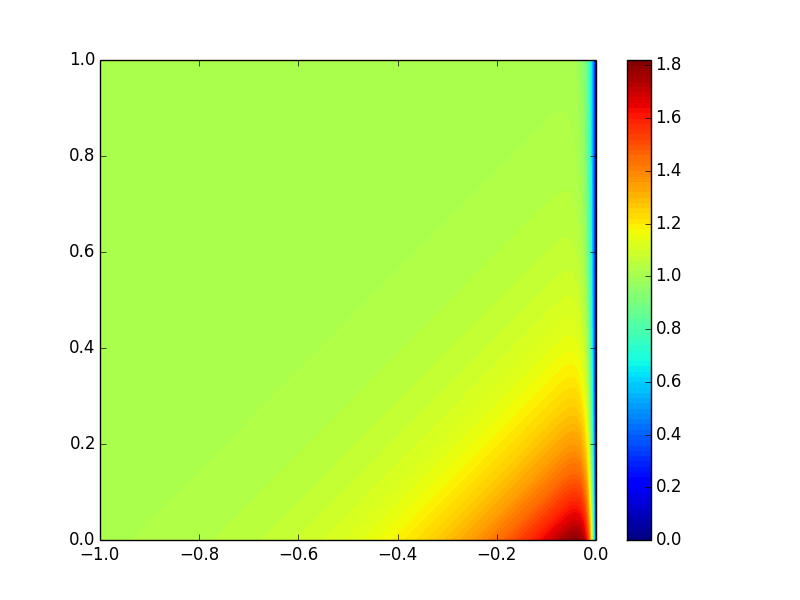
\includegraphics[width=0.8\textwidth]{Confusion/Robustness/1d_problem.png}
\end{figure}
\end{column}
\end{columns}
\end{frame}

% ------------------------------------------------------------
\begin{frame}[t]
\frametitle{Space-Time Convection-Diffusion}
\framesubtitle{$L^2$ Equivalent Norms}
A norm should be: bounded by $\norm{u}_{\LOmega}$, have good conditioning, not produce boundary layers in the optimal test function.
\vspace{-5ex}
\begin{columns}[t]
\begin{column}{0.5\textwidth}
\begin{figure}[t]
\centering
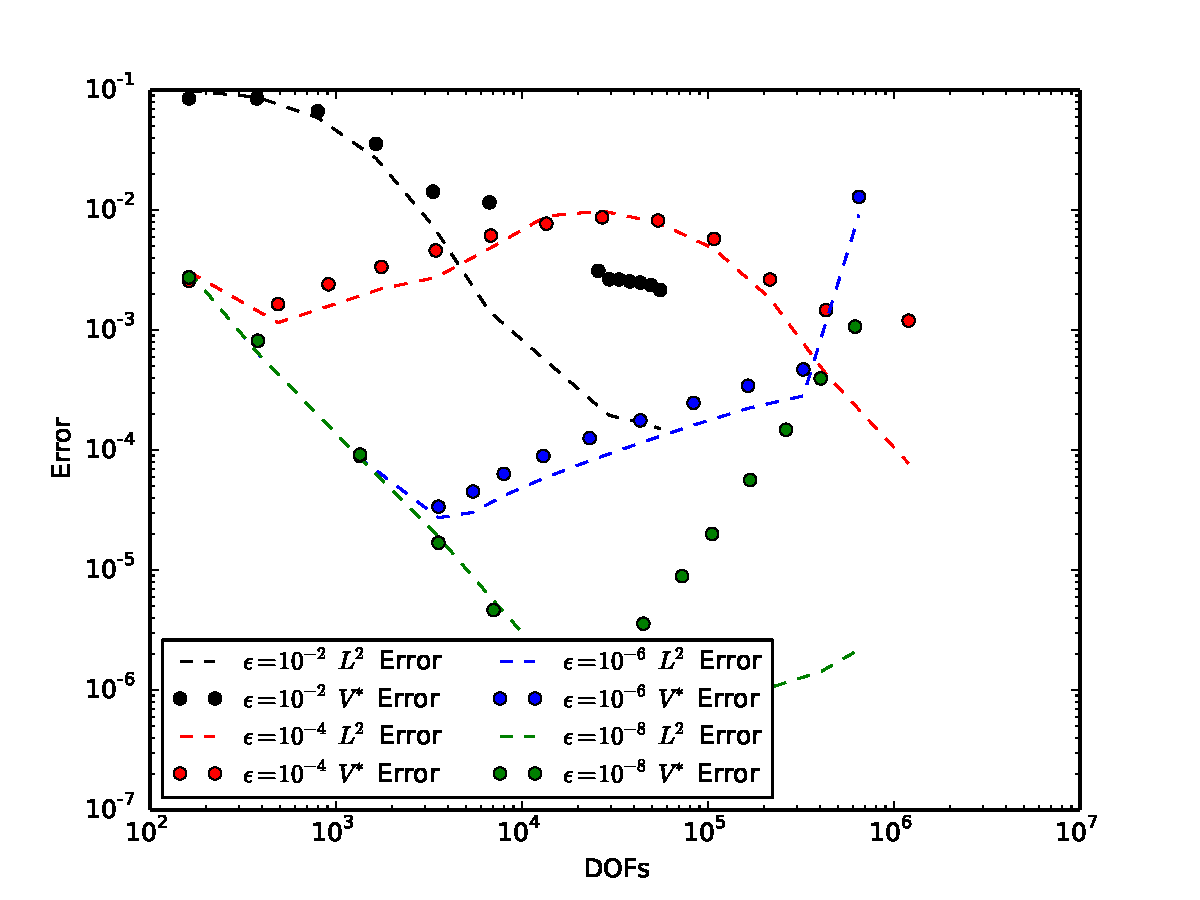
\includegraphics[width=\textwidth]{Confusion/Robustness/convergence1D_p2_graph.pdf}
\end{figure}
\vspace{-5ex}
\small{
\begin{align*}
\norm{(v,\bftau)}^2&=
\norm{\Div\bftau-\tilde\bfbeta\cdot\Gradxt v}^2\\
&+\norm{\frac{1}{\epsilon}\bftau+\Grad v}^2
+\norm{v}^2
+\norm{\bftau}^2
\end{align*}
}
\end{column}
\begin{column}{0.5\textwidth}
\begin{figure}[t]
\centering
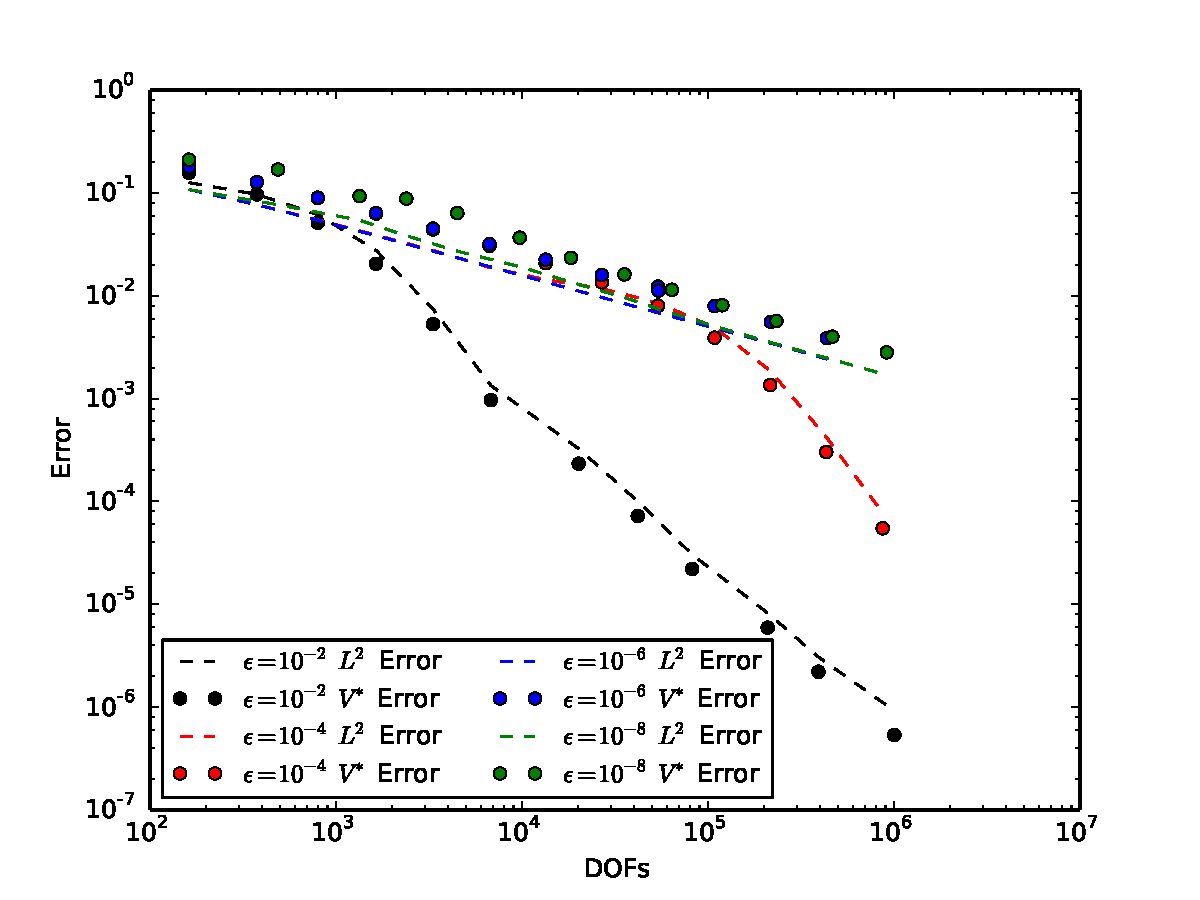
\includegraphics[width=\textwidth]{Confusion/Robustness/convergence1D_p2_robust.pdf}
\end{figure}
\vspace{-5ex}
\small{
\begin{align*}
\norm{(v,\bftau)}^2&=
\norm{\Div\bftau-\tilde\bfbeta\cdot\Gradxt v}^2\\
&+\min\LRp{\frac{1}{h^2},\frac{1}{\epsilon}}\norm{\bftau}^2\\
&+\epsilon\norm{\Grad v}^2
+\norm{\bfbeta\cdot\Grad v}^2
+\norm{v}^2
\end{align*}
}
\end{column}
\end{columns}
\end{frame}

% ------------------------------------------------------------
\begin{frame}[t]
\frametitle{Steady Convection-Diffusion}
\framesubtitle{Ideal Optimal Shape Functions}
\vspace{-3ex}
\begin{columns}
\begin{column}{0.5\textwidth}
\begin{figure}[t]
\centering
Graph Norm
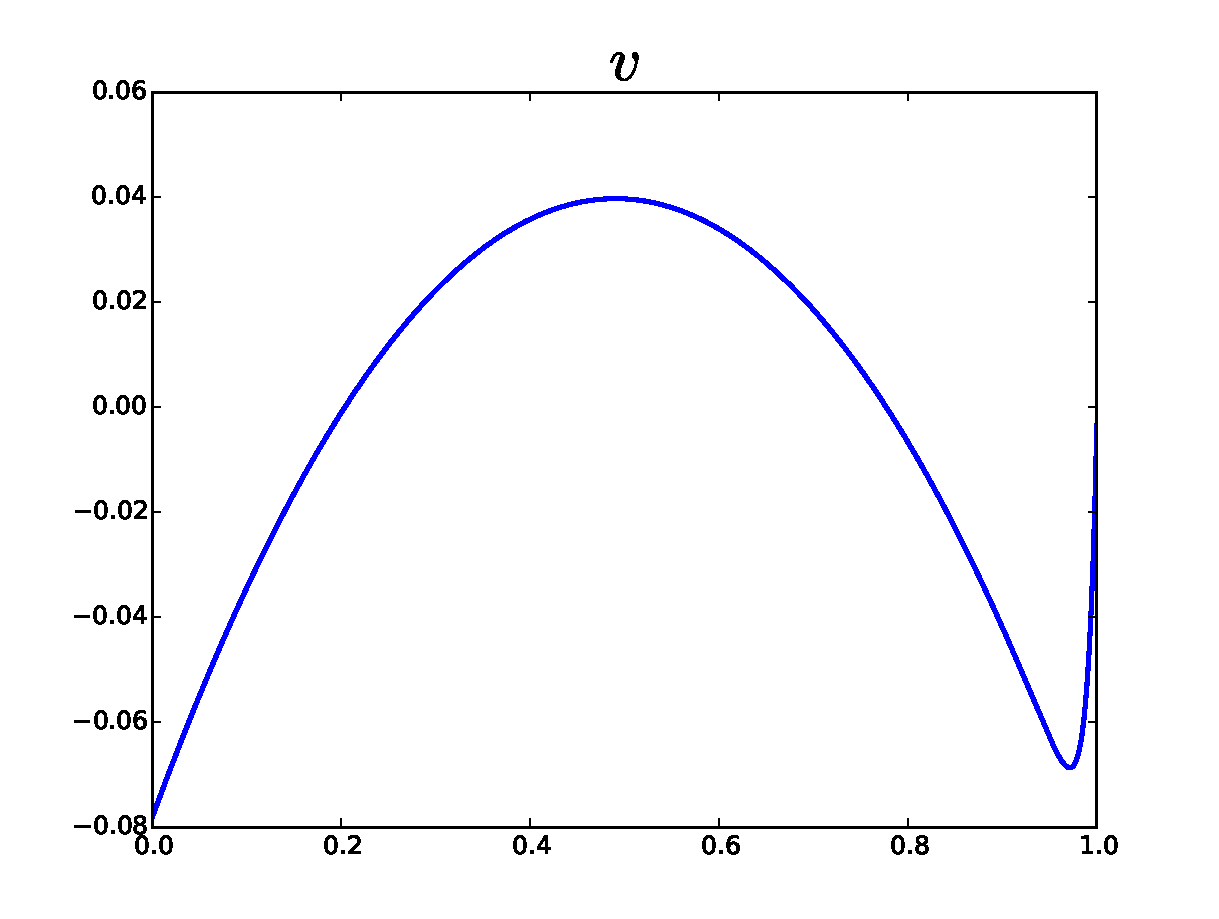
\includegraphics[width=0.8\textwidth]{OptimalTestFunctions/uLinear_1e-2/steady/graph_steady_v.pdf}\\
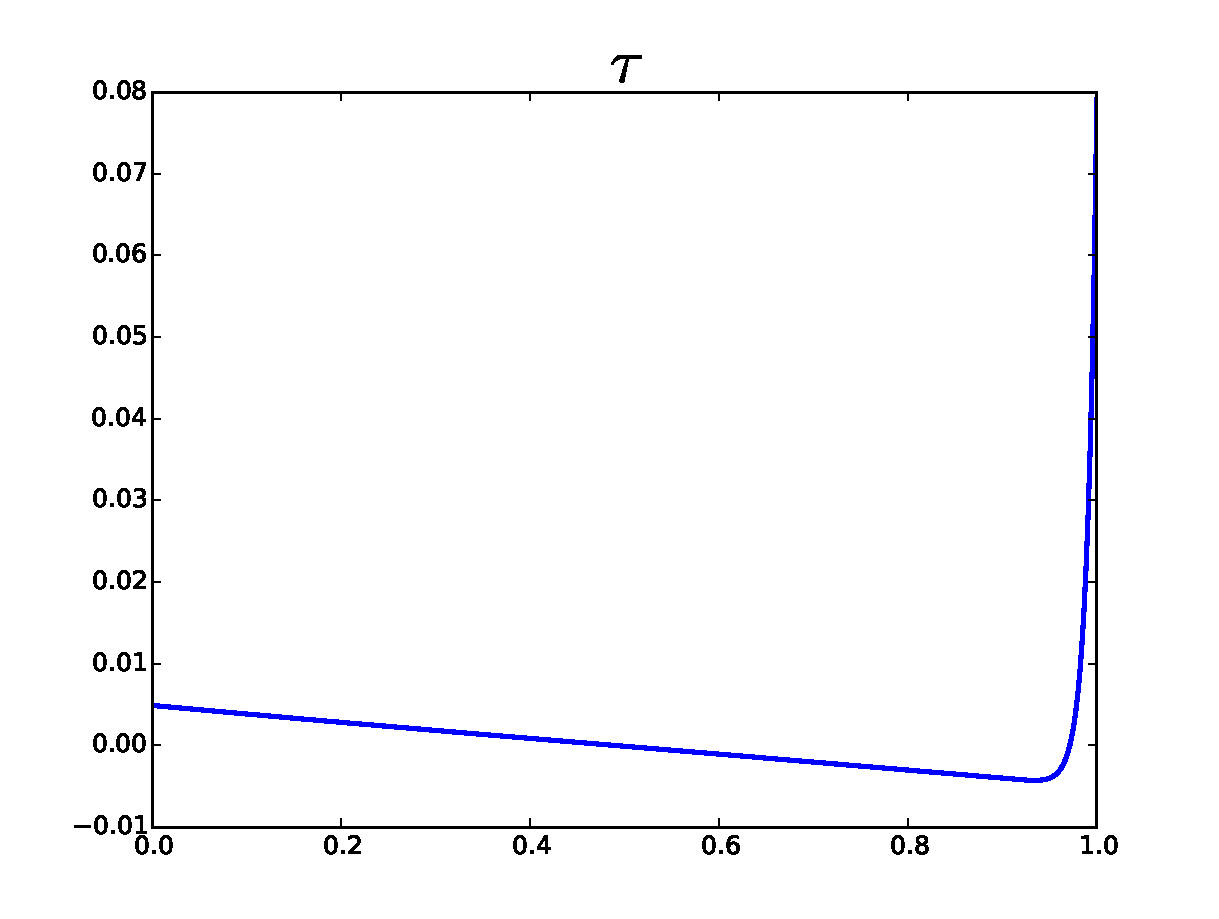
\includegraphics[width=0.8\textwidth]{OptimalTestFunctions/uLinear_1e-2/steady/graph_steady_tau.pdf}
% 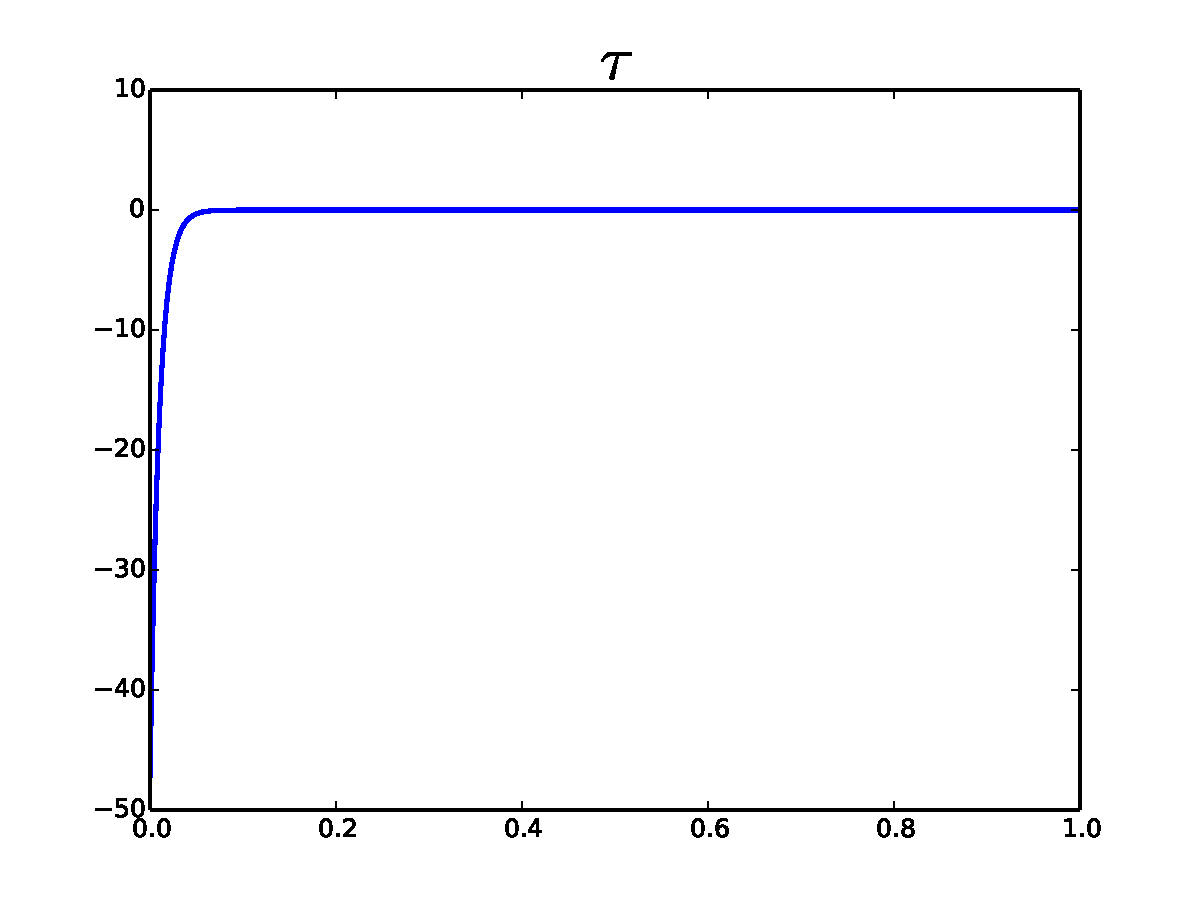
\includegraphics[width=0.8\textwidth]{OptimalTestFunctions/Graph_tau}
\end{figure}
\end{column}
\begin{column}{0.5\textwidth}
\begin{figure}[t]
\centering
Coupled Robust Norm
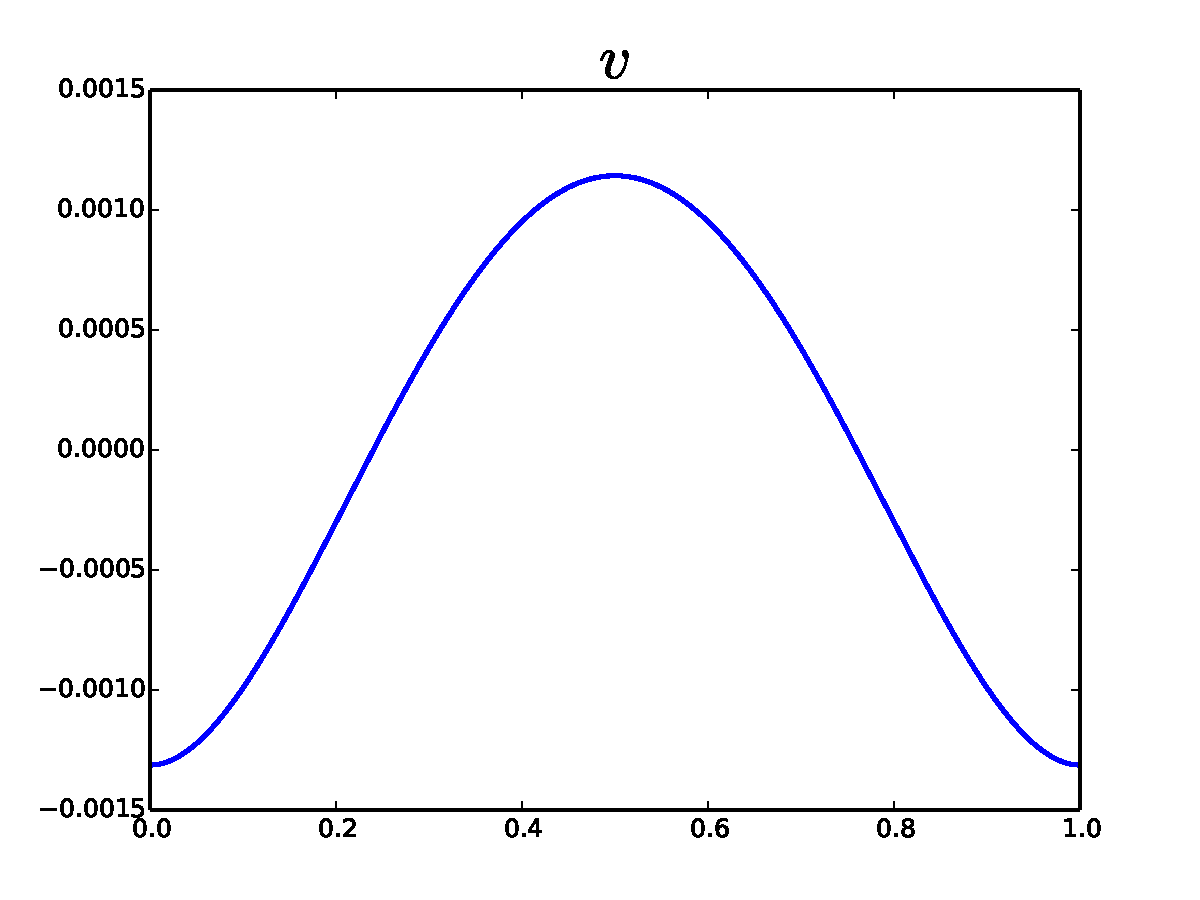
\includegraphics[width=0.8\textwidth]{OptimalTestFunctions/uLinear_1e-2/steady/coupledrobust_steady_v.pdf}\\
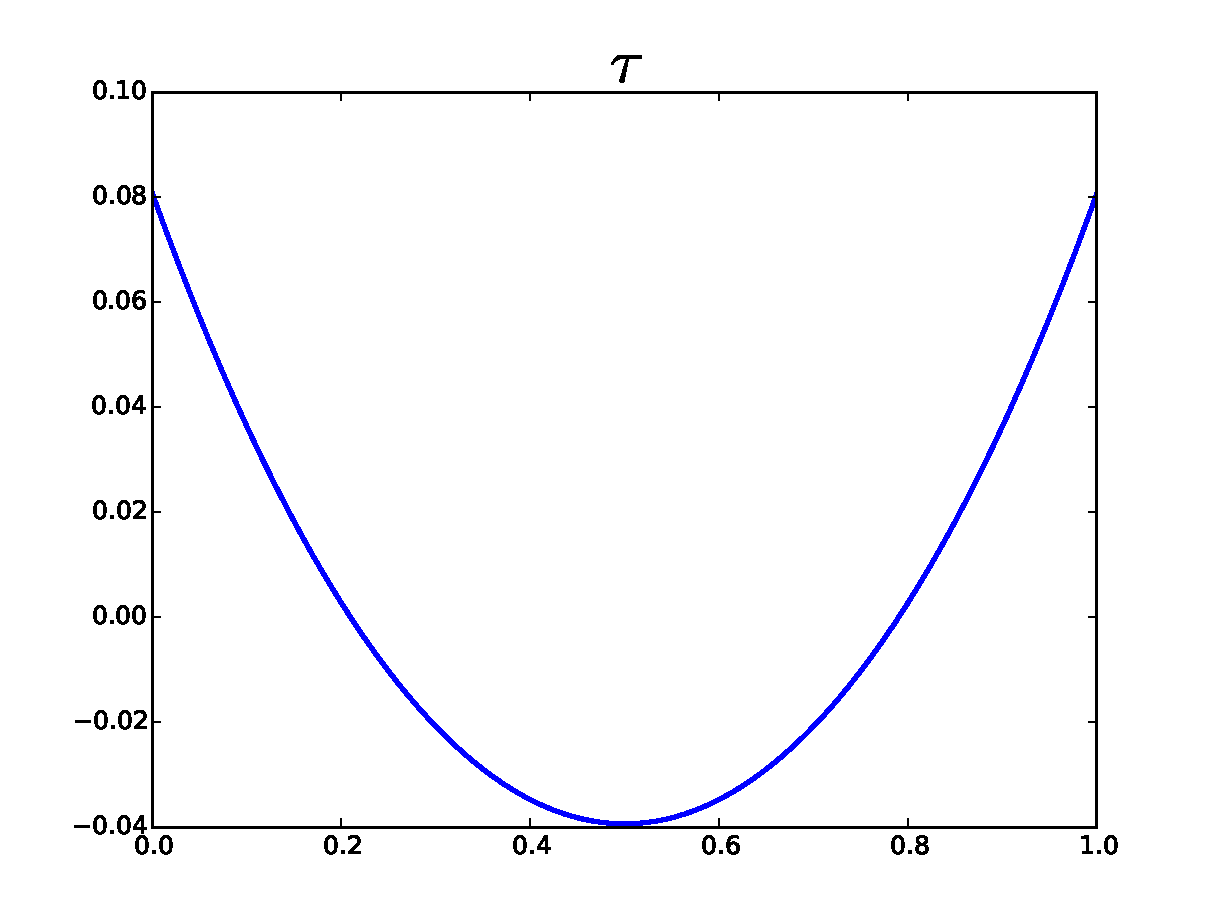
\includegraphics[width=0.8\textwidth]{OptimalTestFunctions/uLinear_1e-2/steady/coupledrobust_steady_tau.pdf}
% 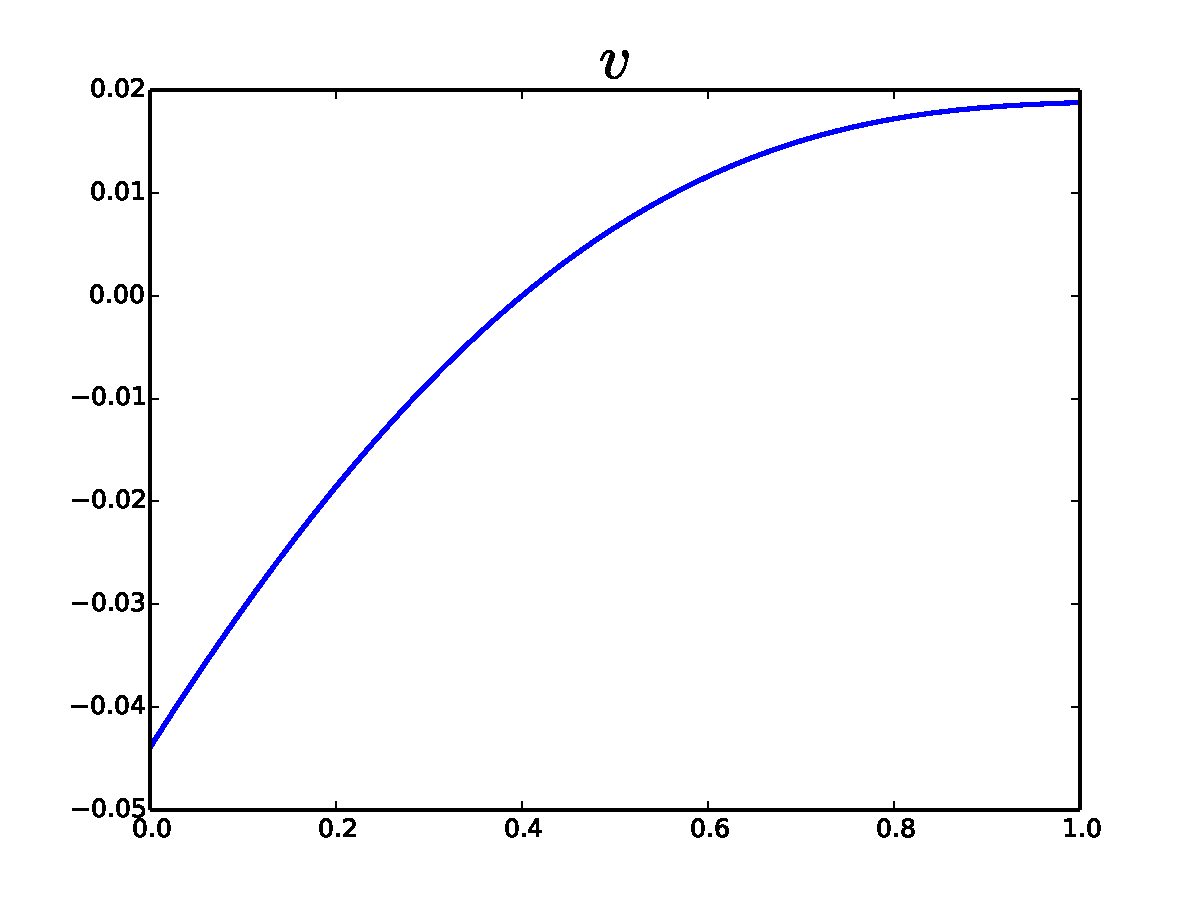
\includegraphics[width=0.8\textwidth]{OptimalTestFunctions/Robust_v}\\
% 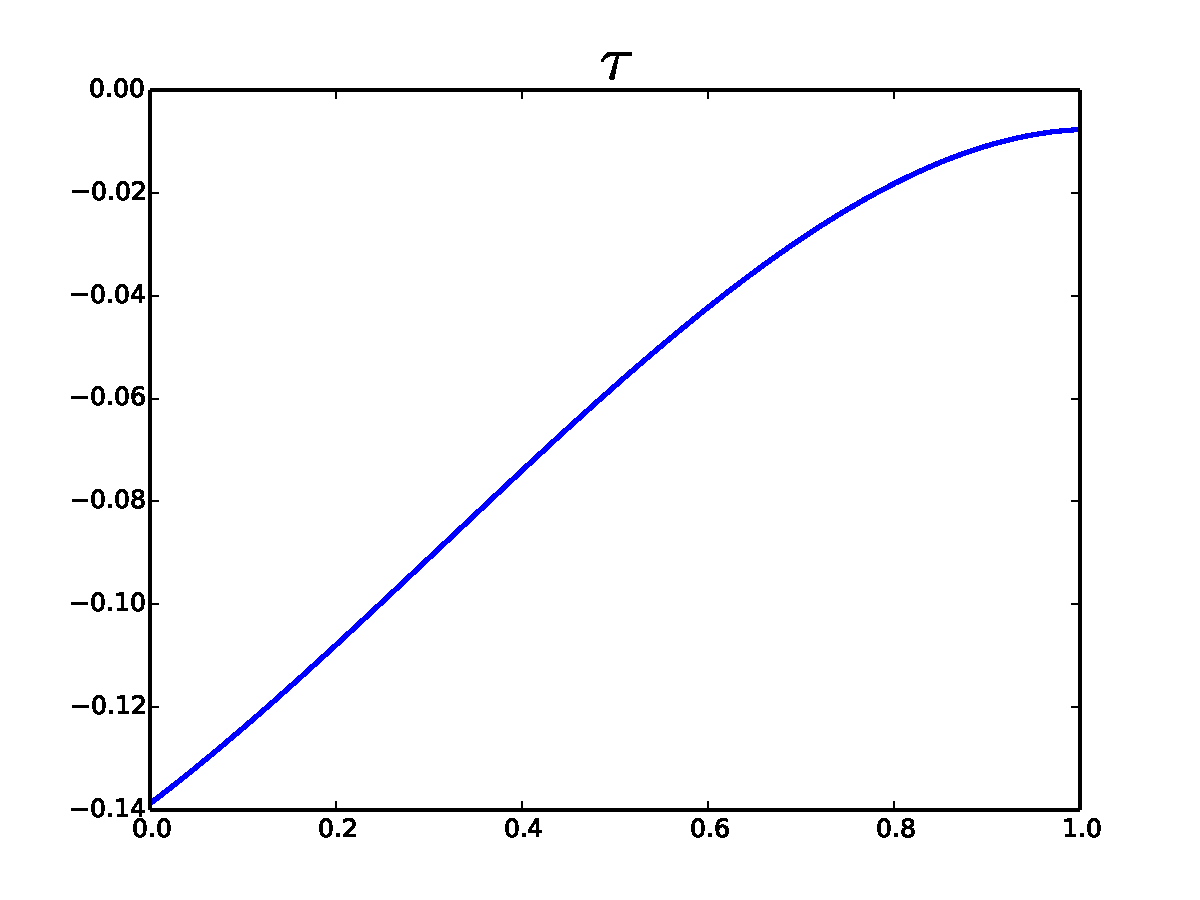
\includegraphics[width=0.8\textwidth]{OptimalTestFunctions/Robust_tau}
\end{figure}
\end{column}
\end{columns}
\end{frame}

% ------------------------------------------------------------
\begin{frame}[t]
\frametitle{Steady Convection-Diffusion}
\framesubtitle{Approximated ($p=3$) Optimal Shape Functions}
\vspace{-3ex}
\begin{columns}
\begin{column}{0.5\textwidth}
\begin{figure}[t]
\centering
Graph Norm
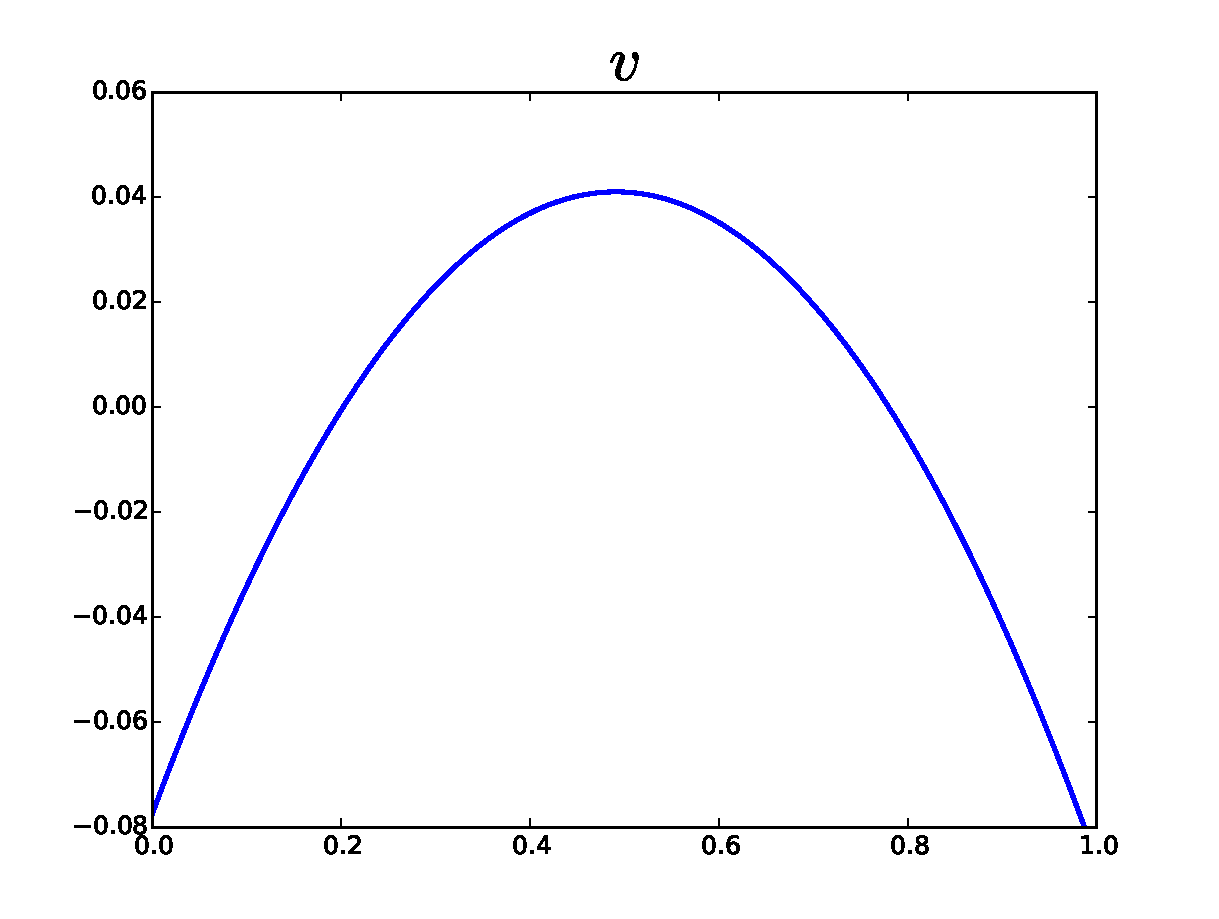
\includegraphics[width=0.8\textwidth]{OptimalTestFunctions/uLinear_1e-2/steady/graph_steady_v_approx3.pdf}\\
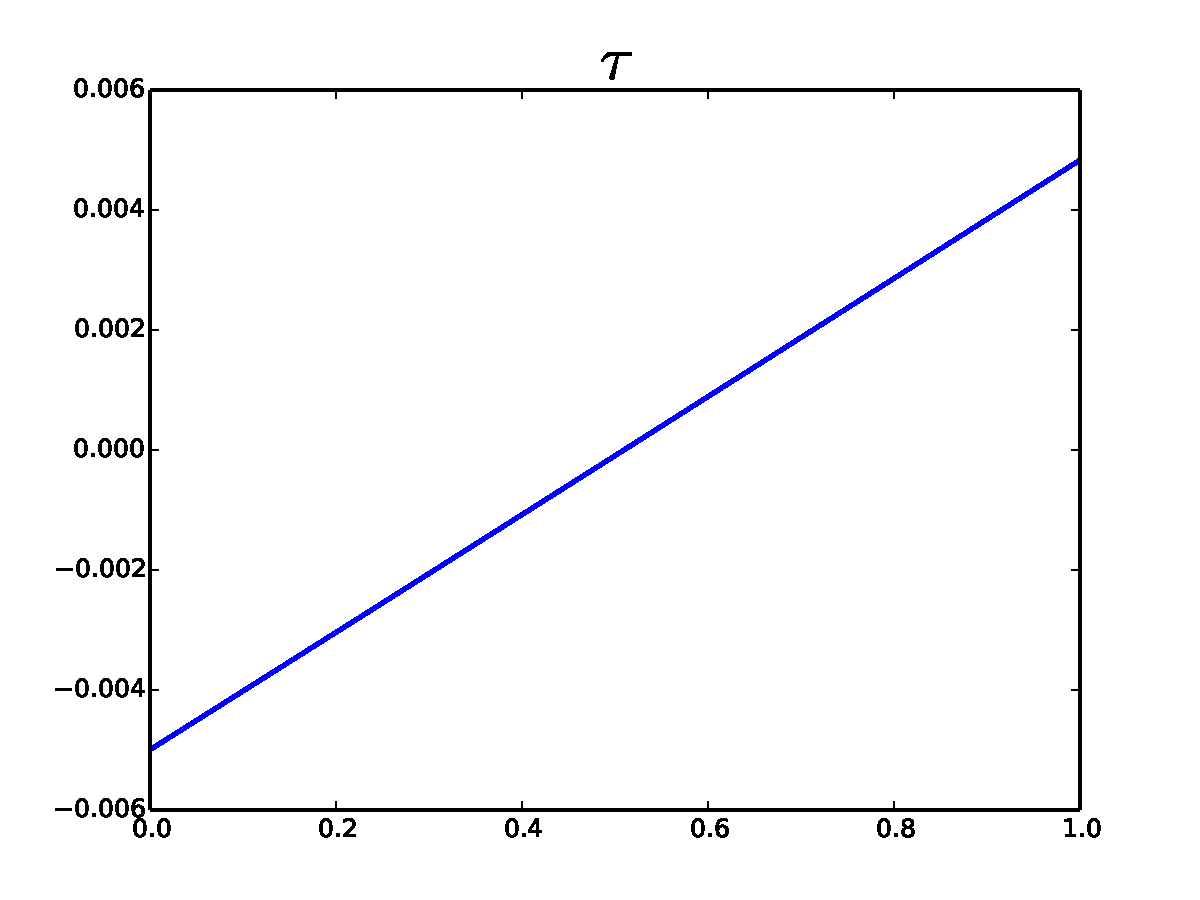
\includegraphics[width=0.8\textwidth]{OptimalTestFunctions/uLinear_1e-2/steady/graph_steady_tau_approx3.pdf}
\end{figure}
\end{column}
\begin{column}{0.5\textwidth}
\begin{figure}[t]
\centering
Coupled Robust Norm
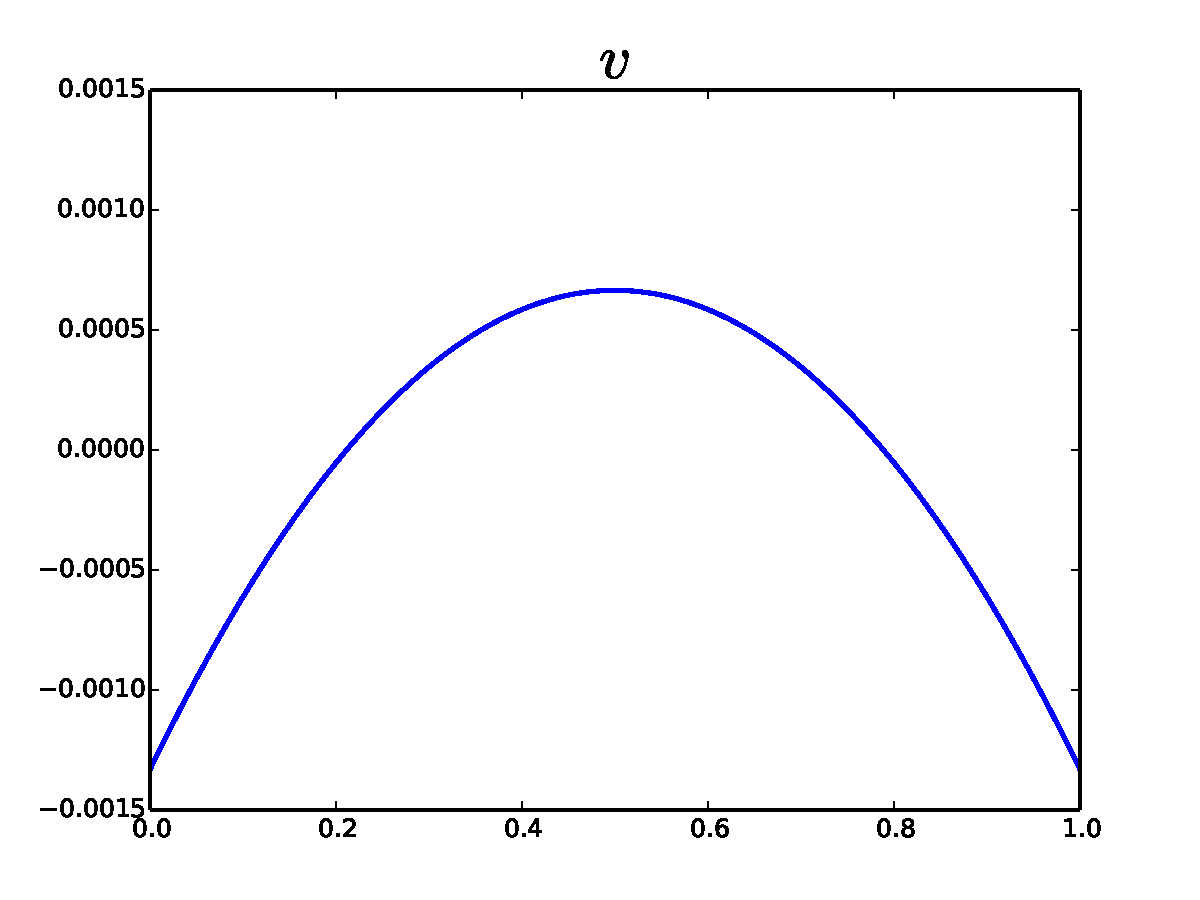
\includegraphics[width=0.8\textwidth]{OptimalTestFunctions/uLinear_1e-2/steady/coupledrobust_steady_v_approx3.pdf}\\
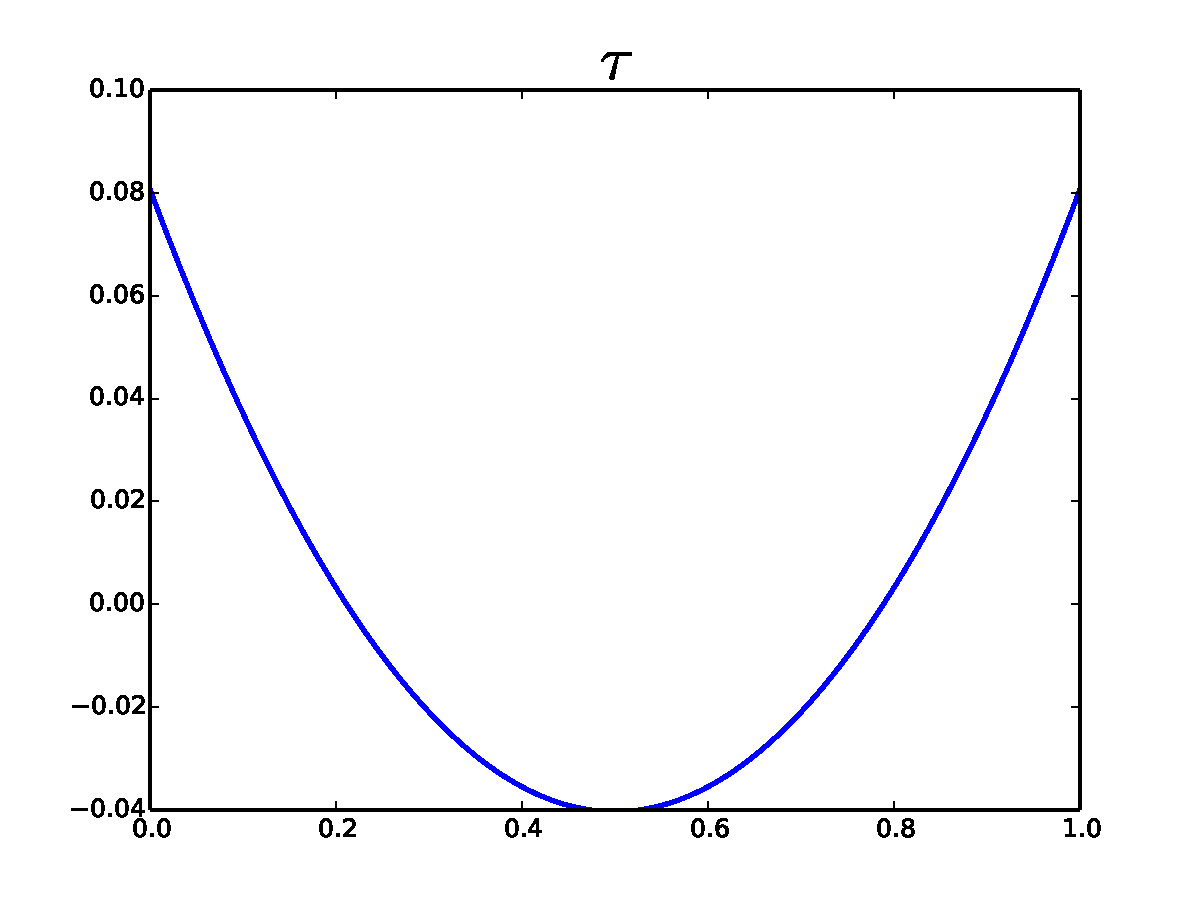
\includegraphics[width=0.8\textwidth]{OptimalTestFunctions/uLinear_1e-2/steady/coupledrobust_steady_tau_approx3.pdf}
\end{figure}
\end{column}
\end{columns}
\end{frame}

% ------------------------------------------------------------
\begin{frame}[t]
\frametitle{Steady Convection-Diffusion}
\framesubtitle{Two Robust Norms for Steady Convection-Diffusion}

The following norms are robust for steady convection-diffusion.

The robust norm was derived in \footfullcite{ChanHeuerThanhDemkowicz2012}:
\begin{align*}
\norm{(v,\bftau)}^2&=
\norm{\bfbeta\cdot\Grad v}^2
+\epsilon\norm{\Grad v}^2
+\min\LRp{\frac{\epsilon}{h^2},1}\norm{v}^2\\
&+\norm{\Div\bftau}^2
+\min\LRp{\frac{1}{h^2},\frac{1}{\epsilon}}\norm{\bftau}^2\,.
\end{align*}
The case for the coupled robust norm was made in \footfullcite{JesseDissertation}:
\begin{align*}
\norm{(v,\bftau)}^2&=
\norm{\bfbeta\cdot\Grad v}^2
+\epsilon\norm{\Grad v}^2
+\min\LRp{\frac{\epsilon}{h^2},1}\norm{v}^2\\
&+\norm{\Div\bftau-\bfbeta\cdot\Grad v}^2
+\min\LRp{\frac{1}{h^2},\frac{1}{\epsilon}}\norm{\bftau}^2\,.
\end{align*}
\end{frame}

% ------------------------------------------------------------
\begin{frame}[t]
\frametitle{Space-Time Convection-Diffusion}
\framesubtitle{Two Robust Norms for Transient Convection-Diffusion}
Let $\tilde\bfbeta:=\vecttwo{\bfbeta}{1}$ and $\Gradxt v:=\vecttwo{\Grad v}{\pd{v}{t}}$.

The following norms are robust for space-time convection-diffusion.

Robust Norm:
\begin{align*}
\norm{(v,\bftau)}^2&=
\norm{\textcolor{red}{\tilde\bfbeta\cdot\Gradxt v}}^2
+\epsilon\norm{\Grad v}^2
+\min\LRp{\frac{\epsilon}{h^2},1}\norm{v}^2\\
&+\norm{\Div\bftau}^2
+\min\LRp{\frac{1}{h^2},\frac{1}{\epsilon}}\norm{\bftau}^2\,.
\end{align*}
Coupled Robust Norm
\begin{align*}
\norm{(v,\bftau)}^2&=
\norm{\textcolor{red}{\tilde\bfbeta\cdot\Gradxt v}}^2
+\epsilon\norm{\Grad v}^2
+\min\LRp{\frac{\epsilon}{h^2},1}\norm{v}^2\\
&+\norm{\Div\bftau-\textcolor{red}{\tilde\bfbeta\cdot\Gradxt v}}^2
+\min\LRp{\frac{1}{h^2},\frac{1}{\epsilon}}\norm{\bftau}^2\,.
\end{align*}
\end{frame}

% ------------------------------------------------------------
\begin{frame}[t]
\frametitle{Robust Norms for Transient Convection-Diffusion}
\framesubtitle{Adjoint Operator}
Consider the problem with homogeneous boundary conditions
\begin{align*}
\frac{1}{\epsilon}\bfsigma-\Grad u &=0\\
\tilde\bfbeta\cdot\Gradxt u - \Div\bfsigma &= f\\
% \Divxt\vecttwo{\bfbeta u-\bfsigma}{u}&=f\\
\beta_n u-\epsilon\pd{u}{n} &= 0 \text{ on } \Gamma_-\\
u &= 0 \text{ on } \Gamma_+\\
u &= u_0 \text{ on } \Gamma_0.
\end{align*}
The adjoint operator $A^*$ is given by 
\[
A^*(v,\bftau)=\LRp{\frac{1}{\epsilon}\bftau+\Grad v,-\tilde\bfbeta\cdot\Gradxt v+\Div\bftau}\,.
\]
\end{frame}

% ------------------------------------------------------------
\begin{frame}[t]
\frametitle{Robust Norms for Transient Convection-Diffusion}
\framesubtitle{Controlling Different Field Variables}
We decompose the continuous adjoint problem
$
A^*(\bftau,v)=(\bfsigma,u)
$
into
\begin{block}{Continuous part with forcing $u$}
\begin{columns}[t]
\begin{column}{0.4\textwidth}
\begin{align*}
\frac{1}{\epsilon}\bftau_1+\Grad v_1 &=0\\
-\tilde\bfbeta\cdot\Gradxt v_1 + \Div\bftau_1 &= u\\
\end{align*}
\end{column}
\begin{column}{0.4\textwidth}
\begin{align*}
\bftau_1\cdot\bfn_x &= 0 \text{ on } \Gamma_-\\
v_1 &= 0 \text{ on } \Gamma_+\\
v_1 &= 0 \text{ on } \Gamma_T
\end{align*}
\end{column}
\end{columns}
\end{block}
\begin{block}{Continuous part with forcing $\bfsigma$}
\begin{columns}[t]
\begin{column}{0.4\textwidth}
\begin{align*}
\frac{1}{\epsilon}\bftau_2+\Grad v_2 &=\bfsigma\\
-\tilde\bfbeta\cdot\Gradxt v_2 + \Div\bftau_2 &= 0\\
\end{align*}
\end{column}
\begin{column}{0.4\textwidth}
\begin{align*}
\bftau_2\cdot\bfn_x &= 0 \text{ on } \Gamma_-\\
v_2 &= 0 \text{ on } \Gamma_+\\
v_2 &= 0 \text{ on } \Gamma_T
\end{align*}
\end{column}
\end{columns}
\end{block}
% % and a continuous part with forcing $\bff$
% \begin{align*}
% \frac{1}{\epsilon}\bftau_2+\Grad v_2 &=\bff\\
% -\tilde\bfbeta\cdot\Gradxt v_2 + \Div\bftau_2 &= 0\\
% \bftau_2\cdot\bfn_x &= 0 \text{ on } \Gamma_-\\
% v_2 &= 0 \text{ on } \Gamma_+\\
% v_2 &= 0 \text{ on } \Gamma_T\,.
% \end{align*}
\end{frame}

% ------------------------------------------------------------
\begin{frame}[t]
\frametitle{Robust Norms for Transient Convection-Diffusion}
\framesubtitle{Proved Bounds at Our Disposal}
Proofs of these lemmas can be found in \footfullcite{EllisRobustnessReport}.
\begin{lemma}[1]
If $\Div\bfbeta=0$, we can bound
\[
\norm{v}^2+\epsilon\norm{\Grad v}^2\leq\norm{u}^2+\epsilon\norm{\bfsigma}^2
\]
where $v=v_1+v_2$.
\end{lemma}
\begin{lemma}[2]
If $\norm{\Grad\bfbeta-\frac{1}{2}\Div\bfbeta\bfI}_{L^{\infty}}\le C_{\bfbeta}$,
we can bound
\[
\norm{\tilde\bfbeta\cdot\Gradxt v_1}\lesssim \norm{u}.
\]
\end{lemma}
\end{frame}

% ------------------------------------------------------------
\begin{frame}[t]
\frametitle{Robust Norms for Transient Convection-Diffusion}
\framesubtitle{Control of $u$}
\begin{block}{Bound on $\norm{(v_1,\bftau_1)}$}
\vspace{-2ex}
\begin{align*}
\text{Lemma (2)}\Rightarrow&&\norm{\tilde\bfbeta\cdot\Gradxt v_1}&\lesssim\norm{u}\\
\text{Lemma (2)}\Rightarrow&&\norm{\Div\bftau_1}&\leq\norm{u}+\norm{\tilde\bfbeta\cdot\Gradxt v_1}\lesssim2\norm{u}\\
\text{Lemma (2)}\Rightarrow&&\norm{\Div\bftau_1-\tilde\bfbeta\cdot\Gradxt v_1}&=\norm{u}\\
\text{Lemma (1)}\Rightarrow&&\norm{v_1}^2+\epsilon\norm{\Grad v_1}^2&\leq\norm{u}^2\\
\text{Lemma (1)}\Rightarrow&&\frac{1}{\epsilon}\norm{\bftau_1}&=\epsilon\norm{\Grad v_1}\leq\norm{u}
\end{align*}
We can guarantee robust control
\[
\norm{(u,0)}_{L^2(\Omega_h)}\lesssim\norm{(u,\bfsigma)}_E\,.
\]
\end{block}
\end{frame}

% ------------------------------------------------------------
\begin{frame}[t]
\frametitle{Robust Norms for Transient Convection-Diffusion}
\framesubtitle{Control of $\bfsigma$}
\begin{block}{Bound on $\norm{(v_2,\bftau_2)}$}
\vspace{-2ex}
\begin{align*}
\text{Definition}\Rightarrow&&\norm{\Div\bftau_2-\tilde\bfbeta\cdot\Gradxt v_2}&=0\leq\norm{\bfsigma}\\
\text{Lemma (1)}\Rightarrow&&\norm{v_2}^2+\epsilon\norm{\Grad v_2}^2&\leq\epsilon\norm{\bfsigma}^2\\
\text{Lemma (1)}\Rightarrow&&\frac{1}{\epsilon}\norm{\bftau_2}&=\norm{\bfsigma}+\epsilon\norm{\Grad v_2}=(1+\epsilon)\norm{\bfsigma}
\end{align*}
We have not been able to prove bounds on $\norm{\tilde\bfbeta\cdot\Gradxt v_2}$ or $\norm{\Div\bftau_2}$. 
\bigskip

We can \textbf{not} guarantee robust control
\[
\norm{(0,\bfsigma)}_{L^2(\Omega_h)}\cancel{\lesssim}\norm{(u,\bfsigma)}_E\,.
\]
\end{block}
\end{frame}

% ------------------------------------------------------------
\begin{frame}[t]
\frametitle{Robust Norms for Transient Convection-Diffusion}
\framesubtitle{Transient Analytical Solution}
Transient impulse decays to Eriksson-Johnson steady state solution.
\[
u=\exp(-lt)\LRs{\exp(\lambda_1 x)-\exp(\lambda_2 x)}+
\cos(\pi y)\frac{\exp(s_1x)-\exp(r_1x)}{\exp(-s_1)-\exp(-r_1)}
\]
\vspace{-4.0ex}
\begin{columns}[t]
\begin{column}{0.3\textwidth}
\begin{figure}[t]
\centering
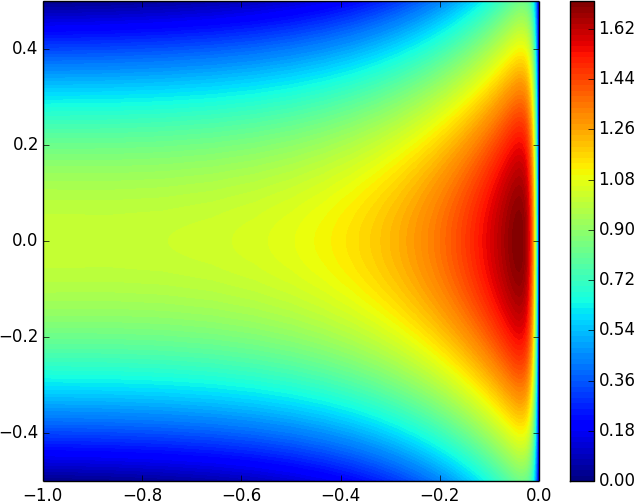
\includegraphics[width=\textwidth]{Confusion/Robustness/2d_problem_t_=_00.png}\\
$t=0.0$
\end{figure}
\end{column}
\begin{column}{0.3\textwidth}
\begin{figure}[t]
\centering
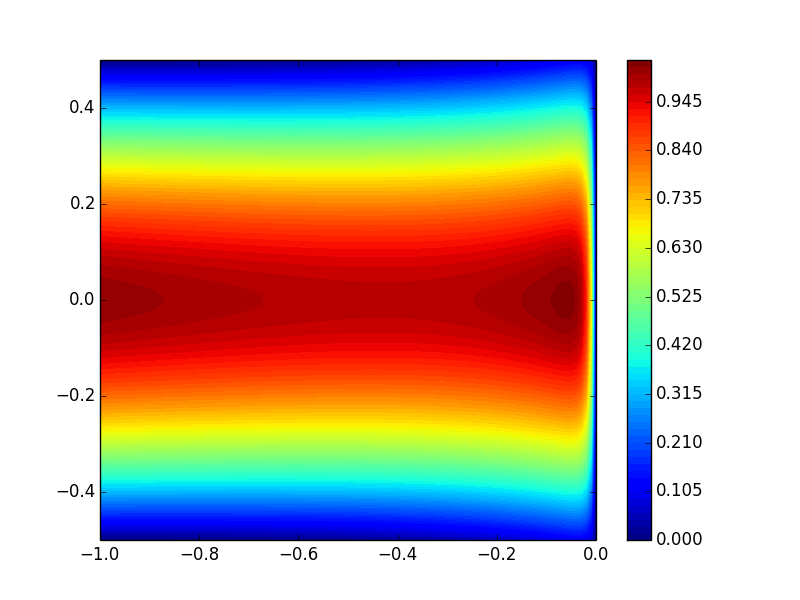
\includegraphics[width=\textwidth]{Confusion/Robustness/2d_problem_t_=_05.png}\\
$t=0.5$
\end{figure}
\end{column}
\begin{column}{0.3\textwidth}
\begin{figure}[t]
\centering
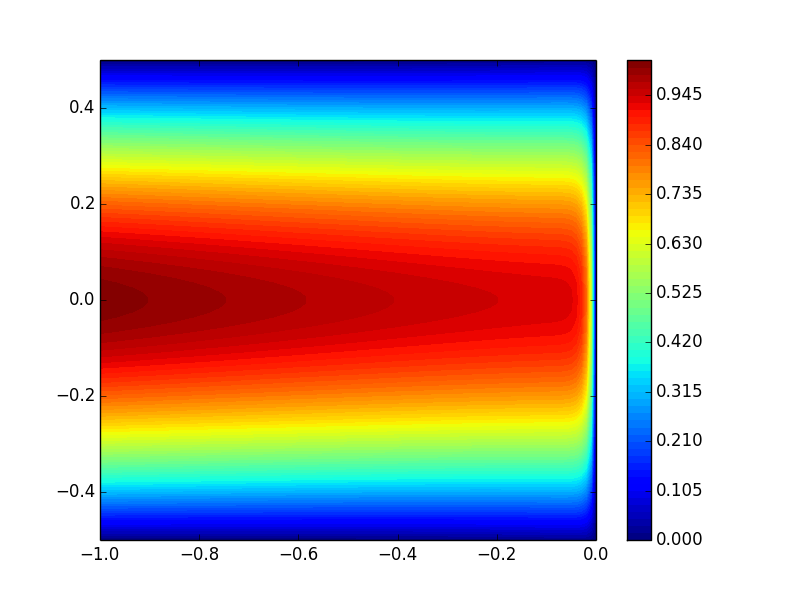
\includegraphics[width=\textwidth]{Confusion/Robustness/2d_problem_t_=_10.png}\\
$t=1.0$
\end{figure}
\end{column}
\end{columns}
\end{frame}

% ------------------------------------------------------------
\begin{frame}[t]
\frametitle{Robust Norms for Transient Convection-Diffusion}
\framesubtitle{Robust Convergence to Analytical Solution}
\vspace{-6.5ex}
\begin{columns}[t]
\begin{column}{0.4\textwidth}
\begin{figure}[t]
\centering
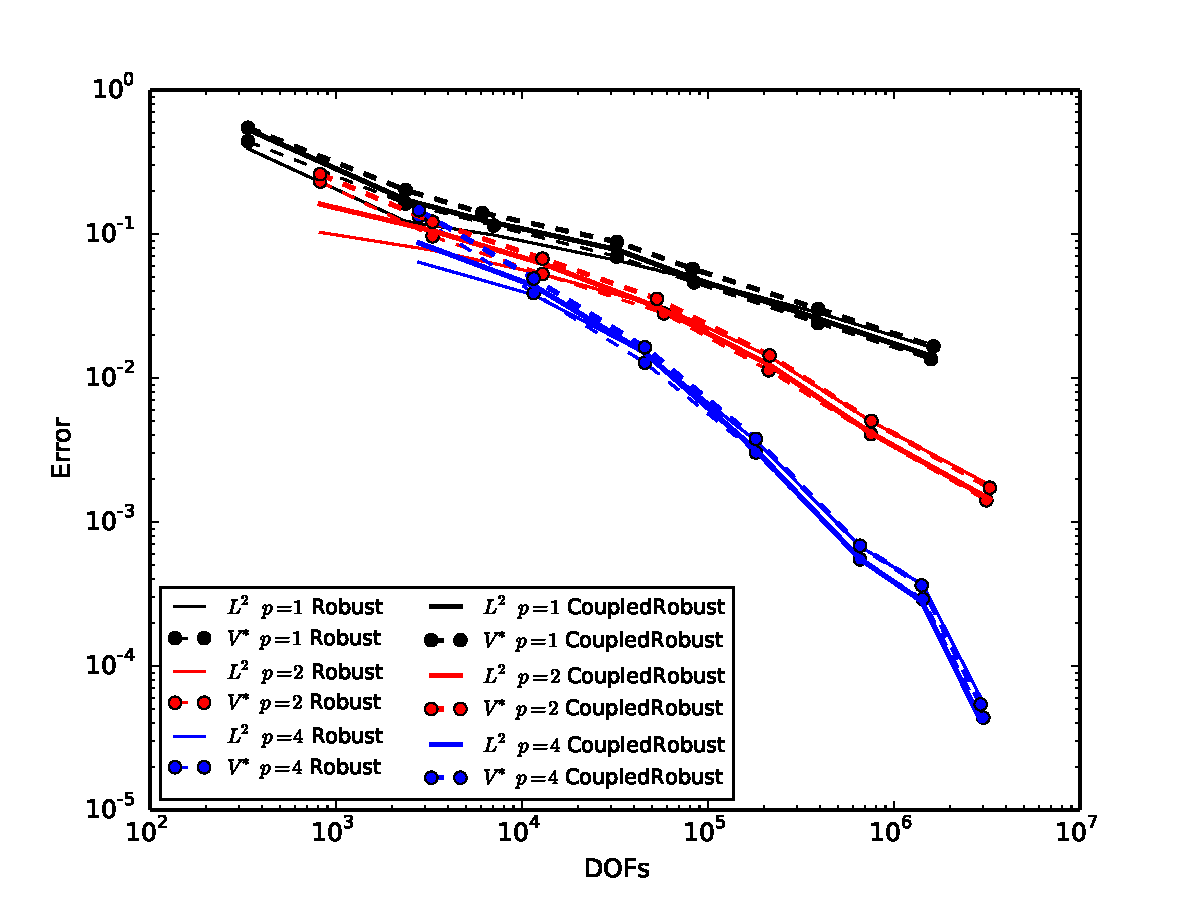
\includegraphics[width=\textwidth]{Confusion/Robustness/convergence_epsilon=1e-2.pdf}\\
\footnotesize{$\epsilon=10^{-2}$}\\
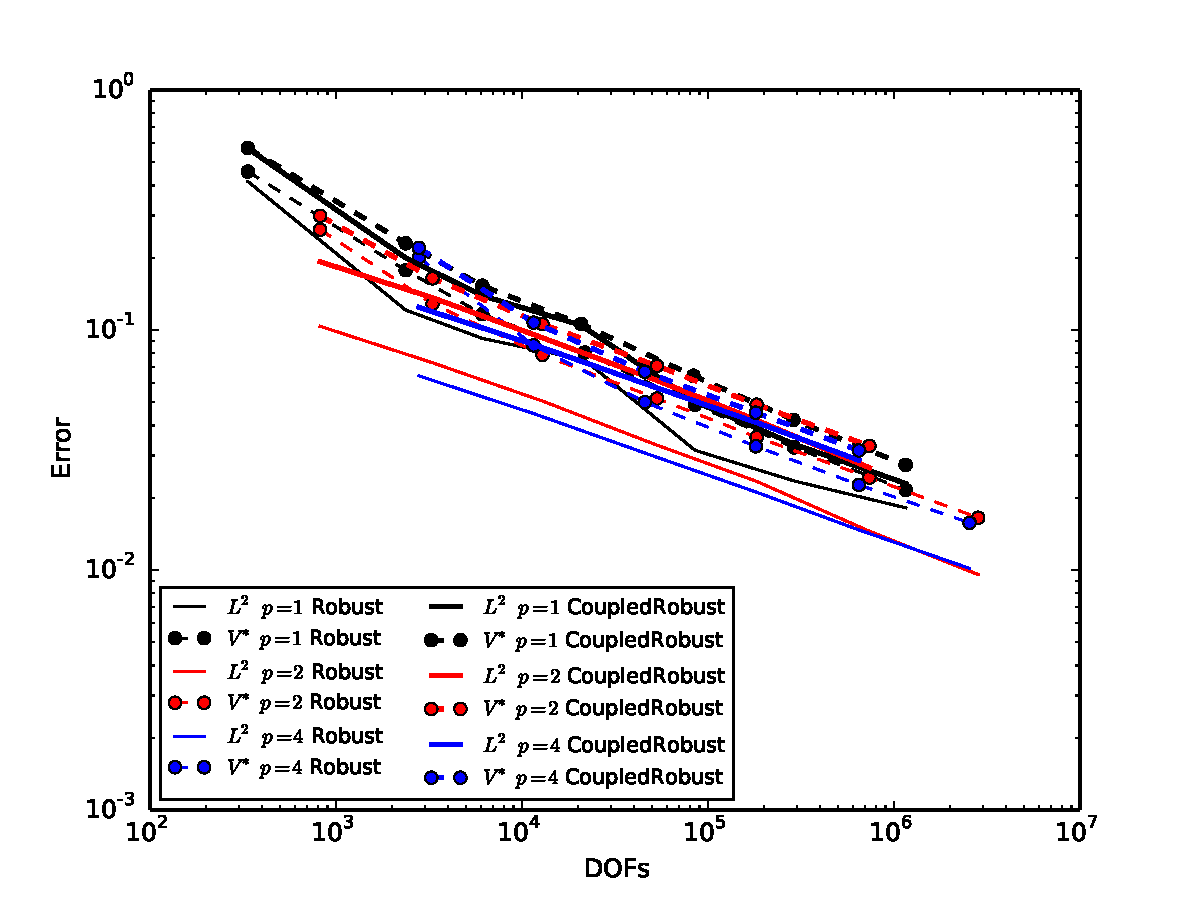
\includegraphics[width=\textwidth]{Confusion/Robustness/convergence_epsilon=1e-6.pdf}\\
\footnotesize{$\epsilon=10^{-6}$}
\end{figure}
\end{column}
\begin{column}{0.4\textwidth}
\begin{figure}[t]
\centering
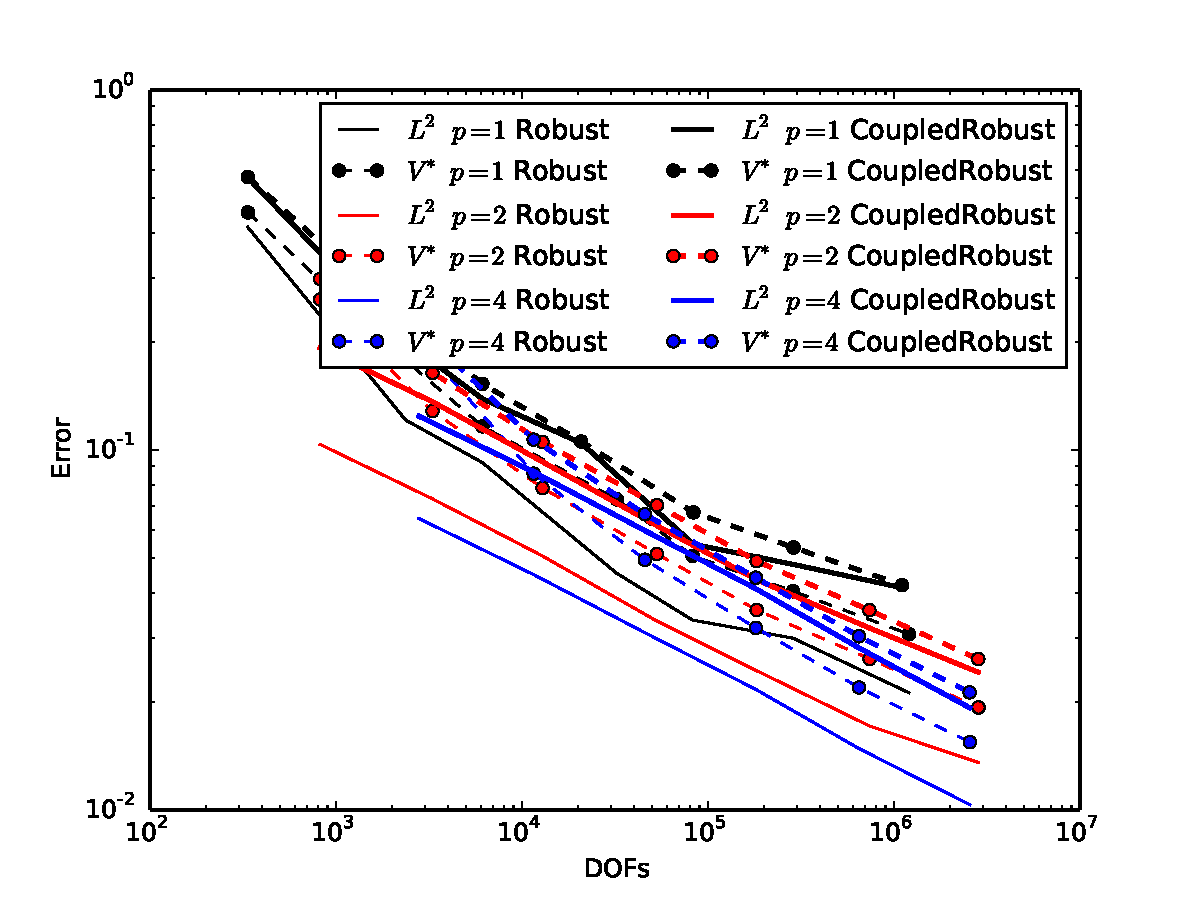
\includegraphics[width=\textwidth]{Confusion/Robustness/convergence_epsilon=1e-4.pdf}\\
\footnotesize{$\epsilon=10^{-4}$}\\
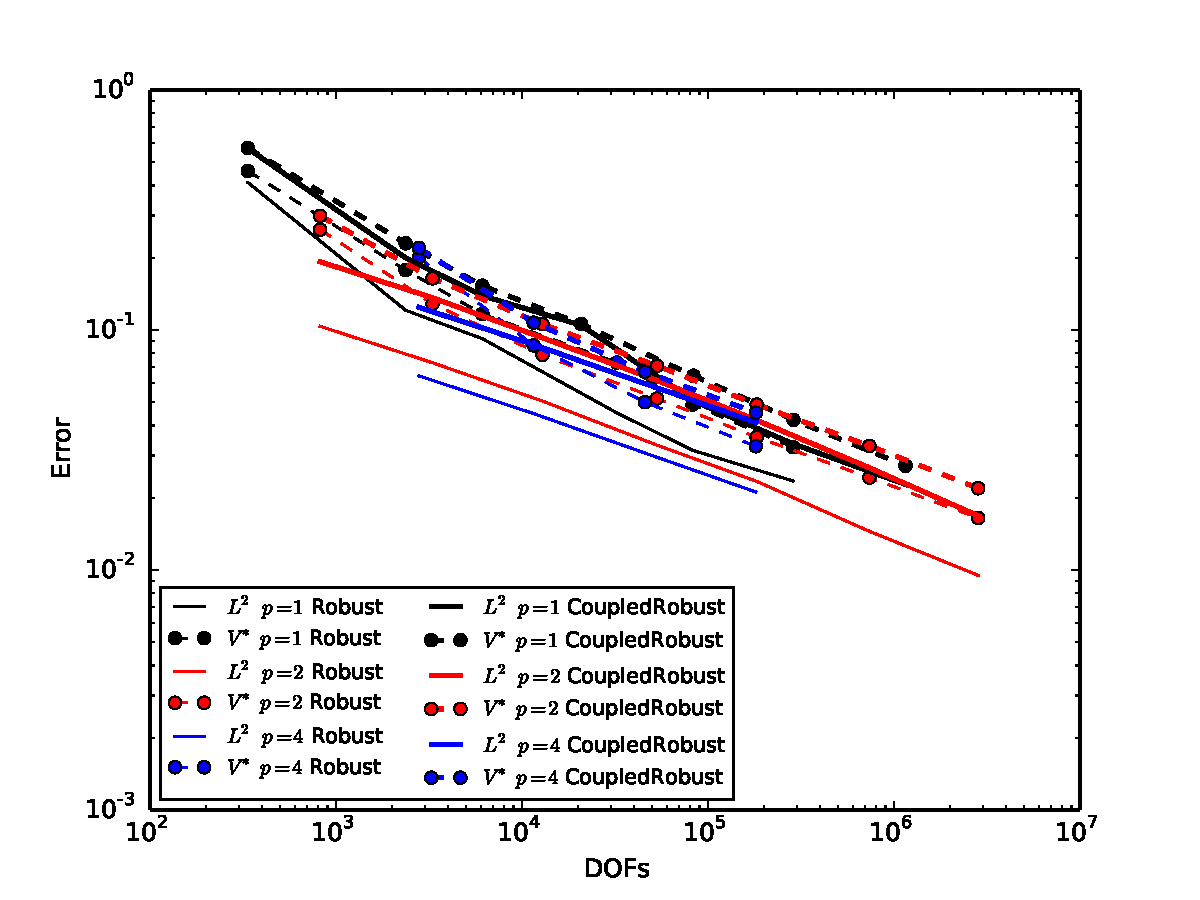
\includegraphics[width=\textwidth]{Confusion/Robustness/convergence_epsilon=1e-8.pdf}\\
\footnotesize{$\epsilon=10^{-8}$}
\end{figure}
\end{column}
\end{columns}
\end{frame}


\begin{frame}[noframenumbering,shrink=10]
\frametitle{Thank You!}
\framesubtitle{Recommended References}
    \nocite{DPGOverview}
    \nocite{DPGEncyclopedia}
    \nocite{EllisRobustnessReport}
    \nocite{CamelliaDPG}
    % \nocite{DemkowiczHeuer}
    % \nocite{ChanHeuerThanhDemkowicz2012}
    \nocite{RobertsDPGNavierStokes}
    \renewcommand*{\bibfont}{\small}
    \setbeamertemplate{bibliography item}[triangle]
    % \printbibliography[keyword=recommended]
    \printbibliography[keyword=main]
    \bigskip
    \printbibliography[notkeyword=main]
\end{frame}

\end{document}
